\chapter{Steife Differentialgleichungen und implizite Verfahren}

\section{Wiederholung: Gewöhnliche Differentialgleichungen und Anfangswertprobleme}

Das folgende Unterkapitel wiederholt ein paar wichtige Konzepte aus dem vorangegangenen
Kapitel.  Es existiert hauptsächlich als Vorlage für eine Vorlesung, die mit steifen
Differentialgleichungen anfängt, und deshalb etwas Vorwissen wiederholen muss.
Beim Lesen dieses Dokuments kann es übersprungen werden.

\bigskip

\subsection{Gewöhnliche Differentialgleichungen}

Gewöhnliche Differentialgleichung:
\begin{equation*}
x'_i=f_i (t,x_1,\ldots,x_d ), \quad i=1,\ldots,d
\end{equation*}
wobei $(t,x) \in \R \times \R^d$ und $f_i \colon \Omega \to \R^d$, $\Omega \subseteq \R \times \R^d$ offen.

\begin{itemize}[nolistsep]
	\item Die Variable $t$ ist häufig als Zeit interpretierbar, man spricht daher häufig von \emph{Evolutionsproblemen}.
	\item $x$ heißt \emph{Zustandsvektor}.
	\item $\R^d$ mit $x \in \R^d$ heißt \emph{Zustandsraum}.
	\item $\R \times \R^d$ heißt \emph{erweiterter Zustandsraum}.
\end{itemize}

\emph{Achtung:} Traditionell verwendet man das gleiche Symbol für Zustände $x \in \R^d$ und Funktionen in den Zustandsraum $x : \R \to \R^d$.  Nicht verwirren lassen!

\paragraph{Beispiele}
\begin{enumerate}
	\item Lineare skalare Differentialgleichung (Radioaktiver Zerfall): Finde $x : \R \to \R$ so dass $x' =-kx$. \\
	\item Allgemeiner: Finde $x : \R \to \R^d$ so dass
	\begin{equation*}
		x' =-Ax,
		\qquad
		A \in \R^{d \times d}.
	\end{equation*}
	\item Höhere Ableitungen können wegtransformiert werden.
	\end{enumerate}

\subsection{Existenz und Eindeutigkeit}

Auch AWPs können mehr als eine Lösung haben.

\begin{bsp}
	Betrachte $x' =\sqrt{\vert x \vert}$, $x(0)=0$. 
	Die Funktion $f(x)=\sqrt{\vert x \vert}$ ist stetig auf $\R$, es existiert also eine Lösung, z.B.: $x(t)=0$ für alle $t$. Eine weitere Lösung ist aber auch $x(t)=\frac{1}{4} t^2$ für $t>0$. Es kommt noch schlimmer:
	Für ein $c>0$, definiere
	\begin{equation*}
	\tilde{x}(t)\colonequals
	\begin{cases}
	0 & \text{falls}\ 0 \leq t \leq c \\
	\frac{1}{4} (t-c)^2 & \text{falls}\ c<t
	\end{cases}
	\end{equation*}
	Auch $\tilde{x}$ löst das Problem. Es gibt also unendlich viele Lösungen!
\end{bsp}


Mit einer einfachen Zusatzforderung an $f$ kann man Eindeutigkeit erhalten.

\begin{defi}
	Die Abbildung $f \in C(\Omega,\R^d)$ heißt auf $\Omega$ bzgl. $x$ lokal \begriff{Lipschitz-stetig}, wenn zu jedem $(t_0,x_0 ) \in \Omega$ ein offener Zylinder 
	\begin{equation*}
		Z \colon (t_0-\tau,t_0+\tau ) \times B_{\rho} (x_0 ) \subset \Omega
	\end{equation*}
	existiert, in dem eine Lipschitzbedingung
	\begin{equation*}
		\vert f(t,x)-f (t,\overline{x} ) \vert \leq L \vert x-\overline{x} \vert
		\qquad
		\forall (t,x),(t,\overline{x} ) \in Z
	\end{equation*}
	mit Konstante $L$ gilt.
\end{defi}

\begin{bem}
	Falls $f(t,x)$ nach $x$ ableitbar ist, dann ist es auch bzgl.\ $x$ lokal Lipschitz-stetig.
\end{bem}

\begin{satz}[Picard--Lindelöf]
	Betrachte das Anfangswertproblem
	\begin{equation*}
		x' = f(t,x) \qquad x(t_0) = x_0
	\end{equation*}
	auf dem erweiterten Zustandsraum $\Omega \subset \R \times \R^d$ mit $(t_0, x_0) \in \Omega$.
	$f$ sei stetig und bzgl. $x$ lokal Lipschitz-stetig.
	
	Dann besitzt das AWP eine eindeutige Lösung.
\end{satz}


\subsection{Evolution und Phasenfluss}

Falls die Bedingungen des Satzes von Picard--Lindelöf gelten, so kann man eine elegante neue Notation einführen.

Sei $(t_0,x_0) \in \Omega$. Bezeichne mit $J_{\max} (t_0,x_0)$ das maximale Zeitintervall, auf dem eine Lösung des dazugehörigen AWPs existiert.
Zu jedem Anfangswert $(t_0,x_0 )$ gibt es eine eindeutige Lösung, d.h. zu jedem AW $(t_0,x_0 )$ ist der Wert $x(t)$ für alle $J_{\max} (t_0,x_0 )$ eindeutig bestimmt.

\begin{defi}
	Für alle $t_0,t \in J_{\max} (t_0,x_0 )$ heißt
	\begin{equation*}
		\Phi^{t,t_0} \colon x_0 \mapsto x(t)
	\end{equation*}
	\begriff{Evolution} der Differentialgleichung $x' = f(t,x)$.
\end{defi}

Die Evolution einer Differentialgleichung ist wohldefiniert, weil das AWP für jedes $x_0$ eine eindeutige Lösung hat. Man kann also schreiben: $x(t) = \Phi^{t,t_0} x_0$.

Für autonome Gleichungen $x'=f(x)$ kann man die Abhängigkeit von $t_0$ weglassen (wähle immer $t_0=0$). Der Evolutionsoperator $\Phi^t x_0=x(t)$ heißt dann \enquote{Phasenfluss}.

\subsection{Das explizite Euler-Verfahren}

\begin{aim}
	Finde eine numerische Approximation der Lösung $x \in C^1 ([t_0,T],\R^d)$ des AWPs
	\begin{equation*}
	x' = f(t,x),
	\qquad
	x(t_0)=x_0
	\end{equation*}
\end{aim}

\emph{Vorgehensweise.}
\begin{itemize}
	\item Unterteile das Intervall $[t_0,T ]$ durch $n+1$ Zeitpunkte
	\begin{equation}
	t_0<t_1<t_2<\ldots<t_n=T.
	\end{equation}
	Die Menge der Zeitpunkte heißt \begriff{Gitter} $\Delta \colonequals \lbrace t_0,t_1,\ldots,t_n \rbrace$
	\item \begriff{Schrittweite}: $\tau_j\colonequals t_{j+1}-t_j$ für $j=0,\ldots,n-1$
	\item Maximale Schrittweite: $\tau_{\Delta}=\max_{j=0,\ldots,n-1} \tau_j$
\end{itemize}

Wir suchen eine Gitterfunktion
\begin{equation*}
	x_{\Delta} \colon \Delta \to \R^d,
\end{equation*}
welche die Lösung des AWPs an den Gitterpunkten möglichst gut approximiert.

\begin{bem}
	Manchmal interpretieren wir so ein $x_\Delta$ auch als eine Funktion $[t_0, T] \to \R^d$, die die Werte an den Gitterpunkten linear interpoliert.
\end{bem}

Unsere Hoffnung ist natürlich, dass für immer feinere Gitter (wenn also $\tau_{\Delta}$ immer kleiner wird) der Unterschied zwischen $x$ und $x_{\Delta}$ immer kleiner wird.

\fbox{\textbf{Das explizite Euler-Verfahren}}
nach \textsc{L. Euler} (1786), auch Eulersches Polygonzugverfahren

\begin{center}
	\begin{overpic}[width=0.5\textwidth]{explicit-euler}
		\put(2,25){$x_0$}
		\put(23,3){$t_0$}
		\put(45,3){$t_1$}
		\put(67,3){$t_2$}
	\end{overpic}
\end{center}

\begin{enumerate}[leftmargin=*]
	\item $x_{\Delta} (t_0)=x_0$
	\item Für $t \in [t_j,t_{j+1} ]$:
	\begin{equation*}
		x_{\Delta} (t)=x_{\Delta} (t_j )+(t-t_j ) f (t_j,x_{\Delta} (t_j ) )
	\end{equation*}
	\item Insbesondere:
	\begin{equation*}
		x_{\Delta} (t_{j+1} )=x_{\Delta} (t_j )+\tau_j f (t_j,x_{\Delta} (t_j ) )
	\end{equation*}
\end{enumerate}

Keine Gleichungsysteme zu lösen $\longrightarrow$ das Verfahren ist explizit.

Beachte: Berechnung durch eine Zweiterm-Rekursion
\begin{enumerate}
	\item $x_{\Delta} (t_0 )=x_0$
	\item $x_{\Delta} (t_{j+1} )=\Psi^{t_{j+1},t_j} x_{\Delta} (t_j ), j=0,1,\ldots,n-1$
\end{enumerate}
mit $\Psi$ unabhängig von $\Delta$.

Die Funktion $\Psi$ heißt \begriff{diskrete Evolution} des expliziten Euler-Verfahrens.


\subsection{Konsistenz}

Der Fehler der Lösung, also der Unterschied $x - x_\Delta$, besteht aus zwei Beiträgen:
\begin{itemize}
	\item Jeder einzelne Schritt produziert einen Fehler.
	\item Da man nach dem ersten Schritt immer von einem fehlerbehafteten Wert startet, bekommt
	man auch falsche Ableitungen $f$.
\end{itemize}

Mit \begriff{Konsistenz} bezeichnet man das \textit{lokale} Verhältnis zwischen der Evolution $\Phi$ und der diskreten Evolution $\Psi$.

\begin{defi}
	Sei $(t,x) \in \Omega$. Die Differenz 
	\begin{equation*}
		\varepsilon (t,x,\tau)=\Phi^{t+\tau,t} x-\Psi^{t+\tau,t} x
	\end{equation*}
	heißt \begriff{Konsistenzfehler} von $\Psi$.
\end{defi}

Eine diskrete Evolution heißt \emph{konsistent}, wenn der Konsistenzfehler keine
konstanten oder linearen Terme in $\tau$ hat. Formaler definiert man das wie folgt:

\begin{defi}
	Eine diskrete Evolution $\Psi$ heißt konsistent, falls
	\begin{alignat*}{2}
	\Psi^{t,t} x & =x &\qquad & \text{für alle $(t,x) \in \Omega$}, \\
	%
	\frac{d}{d \tau} \Psi^{t+\tau,t} x \Big|_{\tau=0} & =f(x,t)
	&& \text{für alle $(t,x) \in \Omega$}.
	\end{alignat*}
\end{defi}


Man kann konsistente Evolutionen einfach charakterisieren. Dazu sei die diskrete Evolution $\Psi^{t+\tau,t} x$ bzgl. $\tau$ stetig differenzierbar. Dann sind äquivalent (\cite[Lemma~4.4]{deuflhard_bornemann:2008}):
\begin{itemize}
	\item $\Psi$ ist konsistent
	\item $\Psi$ hat die Darstellung $\Psi^{t+\tau,t} x=x+\tau \psi (t,x,\tau )$. $\psi$ heißt \begriff{Inkrementfunktion}. $\psi$ ist stetig in $\tau = 0$, und $\psi (t,x,0)=f(t,x)$.
	\item Für den Konsistenzfehler gilt $\varepsilon (t,x,\tau)=o (\tau)$ ($\tau \to 0$).
\end{itemize}

\begin{bsp}
	Das explizite Euler-Verfahrenm $\Psi^{t+\tau,t} x=x+ \tau f(t,x)$ ist konsistent, denn $\frac{\partial \Psi}{\partial \tau} = \frac{\partial}{\partial \tau} (x+ \tau f(t,x))= f(t,x)$.
\end{bsp}

Wir wollen eine \textit{quantitative} Version von Konsistenz.

\begin{defi}
	Eine diskrete Evolution $\Psi$ besitzt Konsistenzordnung $p$, wenn es eine Konstante $C>0$ unabhängig von $t$ und $x$ gibt, so dass
	\begin{equation*}
	\varepsilon (t,x,\tau) \leq C \tau^{p+1}.
	\end{equation*}
\end{defi}

\begin{hinw}
	Ja, der Exponent ist wirklich $p+1$!
\end{hinw}

\begin{bsp}
	Das Euler-Verfahren	hat die Konsistenzordnung $1$.
\end{bsp}


\subsection{Konvergenz}

Konsistenz ist ein lokales Phänomen, d.h. es betrachtet den Fehler nur in der Nähe eines festen $t$. Wir betrachten jetzt, wie gut eine Lösung $x \in C^1 ([t_0,T])$ insgesamt approximiert wird und hoffen, dass für kleinere $\tau_{\Delta}=\max \tau_j$ die Approximation immer besser wird und das schnell!

\begin{defi}
	Der Vektor der Approximationsfehler auf dem Gitter $\Delta$
	\begin{equation*}
		\varepsilon_{\Delta} \colon \Delta \to \R^d,
		\qquad
		\varepsilon_\Delta(t) = x(t)-x_{\Delta}(t)
	\end{equation*}
	heißt \begriff{Gitterfehler}. Seine Norm
	\begin{equation*}
		\Vert \varepsilon_{\Delta} \Vert_{\infty}=\max_{t \in \Delta} \vert \varepsilon_{\Delta} (t) \vert
	\end{equation*}
	heißt \begriff{Diskretisierungsfehler}.
\end{defi}

\begin{defi}
	Zu jedem Gitter $\Delta$ auf $[t_0,T]$ sei eine Gitterfunktion $x_{\Delta}$ gegeben. Die Familie dieser Gitterfunktionen konvergiert mit Ordnung $p \in \N$ gegen $x \in C^1([t_0,T])$, falls eine Konstante $C>0$ existiert, so dass
	\begin{equation*}
		\norm{\varepsilon_{\Delta}}_\infty \leq C \tau_{\Delta}^p
	\end{equation*}
	für alle $\tau_{\Delta}$ klein genug.
\end{defi}

Konvergenz hängt eng mit dem Konsistenzfehler zusammen. Das ist praktisch: Der Konsistenzfehler lässt sich häufig direkt am Verfahren ablesen.

\begin{satz}[{{\cite[Satz~4.10]{deuflhard_bornemann:2008}}}]
	Sei $\psi$ lokal Lipschitz-stetig in $x$. Die diskrete Evolution sei konsistent mit Ordnung $p$, d.h.
	\begin{equation*}
		\varepsilon(t,x,\tau) \colonequals x(t+\tau)-\Psi^{t+\tau,t} x(t)=\mathcal{O} (\tau^{p+1}).
	\end{equation*}
	Dann definiert die diskrete Evolution $\Psi$ für alle Gitter $\Delta$ mit hinreichend kleiner Zeitschrittweite $\tau_{\Delta}$ eine Gitterfunktion $x_{\Delta}$ zum Anfangswert $x_\Delta(t_0) = x_0$.
	Die Familie dieser Gitterfunktionen konvergiert mit Ordnung $p$ gegen die Lösung $x$ des AWPs, d.h.
	\begin{equation*}
		\norm{\varepsilon_{\Delta}}_{\infty}
		\colonequals
		\max_{t \in \Delta} \vert x(t)-x_{\Delta} (t) \vert =\mathcal{O} (\tau_{\Delta}^p)
	\end{equation*}
\end{satz}

\begin{bsp}[Explizites Euler-Verfahren]
	$x_{j+1}=x_j+\tau_j f (t_j,x_j)$
	
	Das Verfahren hat Konsistenzordnung $1$ (der lokale Fehler verhält sich wie $\tau_{\Delta}$). Die Inkrementfunktion $\psi(t,x,\tau) = f(t,x)$ ist lokal Lipschitz-stetig in $x$.
	\begin{itemize}[leftmargin=*]
		\item[$\Rightarrow$] Verfahren konvergiert mit Ordnung $1$, d.h. $\Vert \varepsilon_{\Delta} \Vert_{\infty}=\mathcal{O} (\tau_{\Delta}^1 )$.
		\item[$\Rightarrow$] halber Fehler bedeutet doppelte Anzahl von Zeitschritten.
		\item[$\Rightarrow$] doppelte Anzahl von $f$-Auswertungen $\implies$ doppelter Aufwand
	\end{itemize}
\end{bsp}


\subsection{Explizite Runge--Kutta-Verfahren}

Klassische Konstruktion von Verfahren mit einer höheren Konsistenzordnung.

\emph{Insbesondere}: Hohe Ordnung ohne Ableitungen von $f$

Allgemein hat man ein $s$-stufiges explizites Runge-Kutta-Verfahren:
\begin{enumerate}
	\item $\displaystyle k_i\colonequals f \bigg(t+c_i \tau,x+\tau \sum_{j=1}^{i-1} a_{ij}k_j \bigg)
	\quad \forall i=1,\ldots,s$
	\item $\displaystyle \Psi^{t+\tau,t} x=x+\tau \sum_{i=1}^s b_ik_i$.
\end{enumerate}

Die Größen $k_i=k_i (t,x,\tau )$ heißen \begriff{\emph}{Stufen} des Verfahrens.

Koeffizienten: 
\begin{align*}
	A & = 
	\begin{pmatrix}
	0 \\
	a_{21} & 0 \\
	\vdots & \ddots \\
	a_{s1} & a_{s2} & \ldots & a_{s,s-1} & 0
	\end{pmatrix} \in \R^{s \times s}
	b & = (b_1,\ldots,b_s) \\
	c & = (c_1,\ldots,c_s) \\
\end{align*}
Traditionell notiert man die Koeffizienten im Butcher-Schema:
\begin{center}
	\begin{tabular}{c|c}
		$c^T$ & $A$ \\ \hline
		& $b$
	\end{tabular}
\end{center}

\begin{bsp}
	\begin{itemize}[leftmargin=*]
		\item explizites Euler-Verfahren 
		\begin{tabular}{c|c}
			$0$ & $0$ \\ \hline
			& $1$
		\end{tabular}
		
		\item Verfahren von Runge 
		\begin{tabular}{c|cc}
			$0$ & $0$ &  \\
			$\frac{1}{2}$ & $\frac{1}{2}$ & $0$ \\ \hline
			& $0$ & $1$
		\end{tabular}
		\item Das klassische $4$-stufige Runge-Kutta-Verfahren:
		\begin{center}
			\begin{tabular}{c|cccc}
				$0$ &  &  &  &  \\
				$\frac{1}{2}$ & $\frac{1}{2}$ &  &  &  \\
				$\frac{1}{2}$ & $0$ & $\frac{1}{2}$ &  &  \\
				$1$ & $0$ & $0$ & $1$ &  \\
			\hline
			 & $\frac{1}{6}$ & $\frac{1}{3}$ & $\frac{1}{3}$ & $\frac{1}{6}$ \\
			\end{tabular}
		\end{center}
	\end{itemize}
\end{bsp}

\begin{itemize}
	\item Eine Funktionsauswertung pro Stufe
	\item $s + s + \frac{(s-1)s}{2}$ Parameter bei $s$ Stufen
\end{itemize}

Bei geschickter Wahl der Koeffizienten erhält man Verfahren höherer Ordnung.

\begin{lemma}
	Ein explizites Runge--Kutta-Verfahren ist genau dann konsistent für alle $f \in C(\Omega,\R^d)$, wenn $\sum_{i=1}^s b_i = 1$.
\end{lemma}

Außerdem betrachten wir nur folgende Vereinfachung:

\begin{lemma}
	Ein explizites Runge--Kutta-Verfahren ist genau dann invariant unter Autonomisierung, wenn es konsistent ist, und
	\begin{equation*}
		c_i=\sum_{j=1}^{i-1} a_{ij}
		\qquad
		\text{für $i=1,\dots,s$}
	\end{equation*}
	erfüllt.
\end{lemma}

\section{Steife Differentialgleichungen}

Wir betrachten das explizites Euler-Verfahren
\begin{equation*}
	x_{k+1}=x_k+\tau f \left(t_k,x_k \right)
\end{equation*}
Das Verfahren ist konvergent mit Ordnung $1$.

Löse damit das Anfangswertproblem
\begin{equation*}
	x' =\lambda x \qquad x(0)=1 \qquad (\lambda \in \R)
\end{equation*}

Die folgenden Bilder zeigen Rechnung für $\lambda = 1$, mit verschiedenen Schrittweiten\footnote{Die Tatsache dass die orange Linien nicht bis zum Ende des Zeitintervalls gehen sind Zeichen schlechter Programmierung, aber kein mathematisches Problem.}:

\begin{center}
	\begin{minipage}{0.49\textwidth}
		\centering
		\includegraphics[width=\textwidth]{explicit-euler-lambda-1dot0-h-0dot05}
		\captionof{figure}{$\lambda=1$, $h = 0{,}05$}
	\end{minipage}
	\begin{minipage}{0.49\textwidth}
		\centering
		\includegraphics[width=\textwidth]{explicit-euler-lambda-1dot0-h-0dot1}
		\captionof{figure}{$\lambda=1$, $h = 0{,}1$}
	\end{minipage}
\end{center}

\begin{center}
	\begin{minipage}{0.49\textwidth}
		\centering
		\includegraphics[width=\textwidth]{explicit-euler-lambda-1dot0-h-0dot5}
		\captionof{figure}{$\lambda=1$, $h = 0{,}5$}
	\end{minipage}
	\begin{minipage}{0.49\textwidth}
		\begin{center}
		\includegraphics[width=\textwidth]{explicit-euler-lambda-1dot0-h-1dot0}
		\captionof{figure}{$\lambda=1$, $h = 1{,}0$}
		\end{center}
	\end{minipage}
\end{center}


Als nächstes probieren wir ein negatives $\lambda$, hier z.B.\ $\lambda=-1$:

\begin{center}
\begin{minipage}{0.49\textwidth}
	\centering
	\includegraphics[width=\textwidth]{explicit-euler-lambda--1dot0-h-0dot05} \\
	$\lambda=-1$, $h = 0{,}05$
\end{minipage}
\begin{minipage}{0.49\textwidth}
	\centering
	\includegraphics[width=\textwidth]{explicit-euler-lambda--1dot0-h-0dot1} \\
	$\lambda=-1$, $h = 0{,}1$
\end{minipage}
\end{center}

\begin{center}
	\begin{minipage}{0.49\textwidth}
		\centering
		\includegraphics[width=\textwidth]{explicit-euler-lambda--1dot0-h-0dot5} \\
		$\lambda=-1$, $h = 0{,}5$
	\end{minipage}
	\begin{minipage}{0.49\textwidth}
		\centering
		\includegraphics[width=\textwidth]{explicit-euler-lambda--1dot0-h-1dot0} \\
		$\lambda=-1$, $h = 1{,}0$
	\end{minipage}
\end{center}

\bigskip

Die letzte Rechnung sieht ein wenig seltsam aus, aber der Rest ist okay.

Probieren wir noch $\lambda = -5$:

\begin{center}
	\begin{minipage}{0.49\textwidth}
		\centering
		\includegraphics[width=\textwidth]{explicit-euler-lambda--5dot0-h-0dot05} \\
		$\lambda=-5$, $h = 0{,}05$
	\end{minipage}
	\begin{minipage}{0.49\textwidth}
		\centering
		\includegraphics[width=\textwidth]{explicit-euler-lambda--5dot0-h-0dot1} \\
		$\lambda=-5$, $h = 0{,}1$
	\end{minipage}
\end{center}

\begin{center}
	\begin{minipage}{0.49\textwidth}
		\centering
		\includegraphics[width=\textwidth]{explicit-euler-lambda--5dot0-h-0dot5} \\
		$\lambda=-5$, $h = 0{,}5$
	\end{minipage}
	\begin{minipage}{0.49\textwidth}
		\centering
		\includegraphics[width=\textwidth]{explicit-euler-lambda--5dot0-h-1dot0} \\
		$\lambda=-5$, $h = 1{,}0$
	\end{minipage}
\end{center}
%
Fazit:
\begin{itemize}[topsep=-\parskip, nolistsep]
	\item Keine Überraschungen, falls $\lambda \ge 0$
	\item Falls $\lambda <0$, dann produziert das explizite Euler-Verfahren nur dann qualitativ richtige Ergebnisse, falls der Zeitschritt $\tau < 1/\abs{\lambda}$ ist.
	\item Für $\lambda < 0$, $\tau > 1/\abs{\lambda}$ ist das Verfahren instabil.
\end{itemize}

Rechnen wir diese Beobachtungen nach: Für den expliziten Euler gilt
\begin{equation*}
	x_{k+1}=x_k+\tau f \left(t_k,x_k \right)=x_k+\tau \lambda x_k=\left(1+\lambda \tau \right) x_k=\left(1+\lambda \tau \right)^{k+1}x_0
\end{equation*}

\begin{enumerate}[label=Fall \arabic*:, leftmargin=*]
	\item $\lambda >0$:
	\begin{itemize}[label=--]
		\item Lösung $x(t)=\exp \left(\lambda t \right)$ monoton steigend in $t$
		\item Diskrete Lösung monoton steigend in $k$, da $1+\lambda \tau >1$
	\end{itemize}
	\item $\lambda <0$
	\begin{itemize}[label=--]
		\item Lösung $x(t)=\exp \left(\lambda t \right)$ monoton fallend und positiv
		\item $x_k$ monoton fallend und positiv nur dann, wenn $0<1+\lambda \tau <1 \iff \tau \leq 1/\abs{\lambda}$
	\end{itemize}
	Falls $\lambda < 0$ und $\tau > \frac{1}{\abs{\lambda}}$
	\begin{itemize}[label=--]
		\item Diskrete Lösung oszilliert.
	\end{itemize}
	Falls $\lambda < 0$ und sogar $\tau > \frac{2}{\abs{\lambda}}$
	\begin{itemize}[label=--]
		\item Diskrete Lösung ist unbeschränkt.
	\end{itemize}
\end{enumerate}


\subsection{Steifheit und Kondition}

Für Euler- und Runge-Kutta-Verfahren hatten wir Konvergenzaussagen der Form
\begin{equation*}
	\norm{\varepsilon_\Delta}_\infty\le C \tau_\Delta^p
\end{equation*}
bewiesen.

\emph{Problem:} Diese Aussagen sind \emph{asymptotisch}.
\begin{itemize}
	\item Der Fehler wird kleiner, wenn wir ein hinreichend kleines $\tau_\Delta$ weiter verkleinern.
	%
	\item Die Konstante $C$ ist aber unbekannt: Wir wissen nicht, \emph{wie} klein $\tau_\Delta$ sein muss, um eine vernünftige Genauigkeit zu erzielen. 
	%
	\item Man kann $C$ nur in seltenen Fällen exakt ausrechnen.
\end{itemize}

Wir wollen stattdessen \emph{qualitativ} verstehen, wann $C$ groß sein kann.

Angenommen, wir erhalten für ein gegebenes $\tau_\Delta$ eine gute Approximation der Lösung. 
Dann können wir davon ausgehen, dass das nicht zufällig so ist:  Für einen leicht gestörten Anfangswert $x_0 + \delta x_0$ erwarten wir dann auch eine gute Approximation der gestörten Lösung.


\emph{Erinnerung:} Intervallweise Kondition eines AWPs:
\begin{equation*}
	x'= f(t,x)
	\qquad
	x(t_0) = x_0
	\qquad
	t \in [t_0, T].
\end{equation*}
Eine Störung der Eingabedaten $x_0 \mapsto x_0 + \delta x_0$ führt zu einer Störung der Lösung $x(t) \mapsto x(t) + \delta x(t)$ für alle $t \in [t_0, T]$.

\begin{definition}
	Die \begriff{intervallweise Kondition} $\kappa [t_0,T]$ ist die kleinste Zahl, für die
	\begin{equation*}
		\norm{\delta x}_\infty \le \kappa[t_0,T] \cdot \norm{\delta x_0}.
	\end{equation*}
\end{definition}

Analog führen wir eine \begriff{diskrete Kondition} $\kappa_\Delta$ ein: die Auswirkung einer Störung des Anfangswerts auf eine von einem numerischen Verfahren erzeugte Gitterfunktion
\begin{equation*}
	\norm{\delta x_\Delta}_\infty \le \kappa_\Delta \cdot \norm{\delta x_0}.
\end{equation*}

Wenn ein Verfahren für $x_0$ und $x_0 + \delta x_0$ (mit $\delta x_0$ klein) vernünftige Lösungen liefert, dann muss
\begin{equation*}
	\kappa_\Delta \approx \kappa [t_0, T]
\end{equation*}
gelten.
Umgekehrt bedeutet $\kappa_\Delta \gg \kappa [t_0,T]$, dass das Verfahren völlig unbrauchbar ist, denn es reagiert auf kleine Störungen völlig anders als das eigentliche Problem.
Das Gitter ist dann noch zu grob, da für jedes konvergente Verfahren
\begin{equation*}
	\kappa_\Delta \to \kappa [t_0,T]
	\qquad
	\text{für $\tau_\Delta \to 0$}.
\end{equation*}
gilt.
Die Beziehung
\begin{equation*}
 \kappa_\Delta \approx \kappa [t_0,T]
\end{equation*}
ist eine qualitative Minimalforderung an ein Verfahren und die Wahl des Zeitschritts.
\begin{definition}[Steifheit]
	Für die bisher vorgestellten Verfahren gibt es Anfangswertprobleme, für
	die $\kappa_\Delta \approx \kappa [t_0,T]$ erst für sehr kleine $\tau_\Delta$ gilt.
	Solche Probleme nennt man \begriff{steif}.
\end{definition}

Ungewöhnlich: Es gibt keine mathematisch präzise Definition des Begriffs \enquote{steif}. Eine Verfahrensklasse klassifiziert die Probleme!


\subsection{Beispiel: Das Modellproblem mit explizitem Euler}

Wir betrachten wieder das Modellproblem
\begin{equation*}
	x' = \lambda x,
	\qquad
	x(0) = 1.
\end{equation*}
Wie ist die Kondition dieses AWPs?

Die Lösung des AWPs ist gegeben durch
\begin{equation*}
	x(t) = 1 \cdot e^{\lambda t}.
\end{equation*}

Betrachte jetzt stattdessen einen gestörten Startwert: $x(0)= 1 + d$.
Damit erhalten wir die Lösung
\begin{equation*}
	x(t)= (1+d) \exp ( \lambda t ) = \exp(\lambda t) + d\exp(\lambda t),
\end{equation*}
also ist $\delta x = d \exp ( \lambda t )$ die Störung des Resultats.
Es folgt
\begin{itemize}
	\item $\kappa [0,T] = e^{\lambda T}$ falls $\lambda \ge 0$,
	\item $\kappa [0,T] = 1$ falls $\lambda \le 0$.
\end{itemize}

Die diskrete Kondition des expliziten Euler-Verfahrens
\begin{equation*}
	x_\Delta(t_{k+1})
	=
	(1 + \tau \lambda) x_\Delta(t_k)
	=
	(1+\tau\lambda)^{k+1}x_0
\end{equation*}
ist linear in $x_0$. Deshalb gilt
\begin{equation*}
	\kappa_\Delta = \max_{0\le k \le n -1} \abs{1+\tau \lambda}^{k+1}
\end{equation*}

\begin{enumerate}[label=Fall \arabic*:, leftmargin=*]
	\item $\lambda \ge 0$: Dann ist $\kappa_\Delta = (1+\tau\lambda)^n$.
	Wegen $1 + \tau \lambda \le e^{\tau \lambda}$ gilt
	\begin{equation*}
		\kappa_\Delta = (1+\tau \lambda)^n \le \exp (n \tau \lambda) = e^{\lambda T}
	\end{equation*}
	Also ist $\kappa_\Delta \approx \kappa[0,T]$, das AWP ist nichtsteif.
	%
	\item $\lambda < 0$: 
	\begin{equation*}
		\kappa_\Delta = \max_{0 \le k \le n -1} \abs{1 - \tau_\Delta \abs{\lambda}}^{k+1}
	\end{equation*} 	
	Falls $\tau < \frac{2}{\abs{\lambda}}$ so ist $\kappa_\Delta \le 1 = \kappa[0,T]$.
	Andererseits gilt für $\tau_\Delta \gg 2 / \abs{\lambda}$
	\begin{equation*}
		\kappa_\Delta = \abs{1-\tau \abs{\lambda}}^n \gg 1 = \kappa [0,T].
	\end{equation*}
	Das Problem ist steif.
\end{enumerate}

\subsection{Stabilität}

Wir betrachten noch einmal das vorige gestörte AWP
\begin{equation*}
	x' = \lambda x,
	\qquad
	x(0) = 1 + d
\end{equation*}
Wie verhält sich die Störung $d \exp (\lambda t)$? Dazu betrachten wir die drei Fälle:
\begin{enumerate}[label=Fall \arabic*:, leftmargin=*]
	\item $\lambda>0$: Die Störung wächst exponentiell mit $t$. Das Lösen der Gleichung für große $t$ ist kaum sinnvoll, bzw. sehr schwierig.
	\item $\lambda=0$: Die Störung bleibt für alle $t$ in konstanter Größe erhalten.
	\item $\lambda<0$: Für große $t$ wird die Störung \enquote{von alleine} immer kleiner!
\end{enumerate}

Betrachtet man die Auswirkung von Störungen nicht auf ein beschränktes Intervall $[t_0,T]$, sondern für alle Zeiten $[t_0,\infty)$, dann spricht man statt von Kondition meistens von \begriff{Stabilität}.

Die obige Dreiteilung ist typisch. Wir machen daraus eine Definition.

\begin{defi}
	Sei $\left(t_0,x_0 \right)$ so, dass $\Phi^{t,t_0} x_0$ für alle $t \geq t_0$ existiert. Die Lösung des AWPs heißt
	\begin{enumerate}[label=(\arabic*)]
		\item \begriff{instabil}, falls weder (2) noch (3) gelten.
		\item \begriff{(Lyapunov)-stabil}, falls zu jedem $\varepsilon >0$ ein $\delta >0$ existiert, so dass
		\begin{equation*}
			\big\Vert \Phi^{t,t_0} x -\Phi^{t,t_0} x_0 \big\Vert \leq \varepsilon
		\end{equation*}
		für alle $t \geq t_0$ und $\left\Vert x-x_0 \right\Vert \leq \delta$,
		\item \begriff{asymptotisch stabil}, falls es zusätzlich ein $\delta_0>0$ gibt, so dass
		\begin{equation*}
			\lim_{t \to \infty} \big\Vert \Phi^{t,t_0} x -\Phi^{t,t_0} x_0 \big\Vert =0
		\end{equation*}
		falls $\Vert x-x_0 \Vert \leq \delta_0$,
	\end{enumerate}
\end{defi}

\begin{bem}
	Dieser Stabilitätsbegriff hat nichts mit der Stabilität von Algorithmen zu tun.
	Es kann anspruchsvoll bis zu schwierig sein, die Stabilität von DGL zu bestimmen.
\end{bem}


\subsection{Das implizite Euler-Verfahren}

Expliziter Euler: 
\begin{equation*}
	x_{k+1}=x_k+\tau f \left(t_k,x_k \right)
\end{equation*}
Impliziter Euler: 
\begin{equation*}
	x_{k+1}=x_k+\tau f \left(t_{k+1},x_{k+1} \right)
\end{equation*}
Implizit bedeutet, dass in jedem Schritt ein Gleichungssystem gelöst werden muss.

Betrachten wir wieder das AWP
\begin{equation*}
	x' =\lambda x\qquad x(0)=1\qquad (\lambda \in \R)
\end{equation*}
Implizites Euler-Verfahren: 
\begin{align*}
	x_{k+1} & =x_k+\tau f \left(t_{k+1},x_{k+1} \right)=x_k+\tau \lambda x_{k+1} \\
	\implies x_{k+1} & =\frac{x_k}{1-\tau \lambda}=\left(\frac{1}{1-\tau \lambda} \right)^{k+1}x_0
\end{align*}
Wenn $\lambda <0$, so ist 
\begin{equation*}
	0<\frac{1}{1-\tau \lambda} <1
\end{equation*}
für alle $\tau >0$. Das Verfahren ist für alle $\tau > 0$ stabil.

Das probieren wir wieder numerisch aus. Hier ist das implizite Euler-Verfahren
für $x' = \lambda x$ mit $\lambda = -5$:

\begin{center}
	\begin{minipage}{0.49\textwidth}
		\centering
		\includegraphics[width=\textwidth]{implicit-euler-lambda--5dot0-h-0dot05} \\
		$\lambda=-5$, $h = 0{,}05$
	\end{minipage}
	\begin{minipage}{0.49\textwidth}
		\centering
		\includegraphics[width=\textwidth]{implicit-euler-lambda--5dot0-h-0dot1} \\
		$\lambda=-5$, $h = 0{,}1$
	\end{minipage}
\end{center}

\begin{center}
	\begin{minipage}{0.49\textwidth}
		\centering
		\includegraphics[width=\textwidth]{implicit-euler-lambda--5dot0-h-0dot5} \\
		$\lambda=-5$, $h = 0{,}5$
	\end{minipage}
	\begin{minipage}{0.49\textwidth}
		\includegraphics[width=\textwidth]{implicit-euler-lambda--5dot0-h-1dot0} \\	
		$\lambda=-5$, $h = 1{,}0$
	\end{minipage}
\end{center}

Die letzte Rechnung (mit $h=1{,}0$) ist zwar nicht mehr sonderlich präzise,
aber stabil ist sie.

Ist jetzt alles gut?  Nein, denn es steht zu vermuten dass wir für positive $\lambda$ Probleme kriegen.  Und in der Tat, für $\lambda = 1$ sieht das Ergebnis nicht mehr so rosig aus:

\begin{center}
	\begin{minipage}{0.49\textwidth}
		\centering
		\includegraphics[width=\textwidth]{implicit-euler-lambda-1dot0-h-0dot05} \\
		$\lambda=1$, $h = 0{,}05$
	\end{minipage}
	\begin{minipage}{0.49\textwidth}
		\centering
		\includegraphics[width=\textwidth]{implicit-euler-lambda-1dot0-h-0dot1} \\
		$\lambda=1$, $h = 0{,}1$
	\end{minipage}
\end{center}
\begin{center}
	\begin{minipage}{0.49\textwidth}
		\centering
		\includegraphics[width=\textwidth]{implicit-euler-lambda-1dot0-h-0dot5} \\
		$\lambda=1$, $h = 0{,}5$
	\end{minipage}
	\begin{minipage}{0.49\textwidth}
		\centering
		\includegraphics[width=\textwidth]{implicit-euler-lambda-1dot0-h-0dot8} \\
		$\lambda=1$, $h = 0{,}8$
	\end{minipage}
\end{center}

Man beachte hier die wechselnde Skalierung der vertikalen Achse.  Die Zeitschrittweite im letzten Bild ist $0{,}8$ statt wie bisher $1{,}0$, weil der Wert $1{,}0$ im Verfahren zu einer Division durch Null führt.


\section{Stabilität von Einschrittverfahren}

Das explizite Euler-Verfahren wird für die lineare Gleichung
\begin{equation*}
	x' = \lambda x, \qquad x(t_0) = x_0
\end{equation*}
instabil, wenn $\lambda <0$ und der Zeitschritt $\tau$ zu groß ist.

\subsection{Stabilität von linearen, autonomen, homogenen Differentialgleichungen}

Wir verallgemeinern das jetzt und betrachten \textit{lineare}, autonome, homogene Systeme
\begin{equation*}
	x' = Ax \qquad x(0)=x_0 \in \R^d \qquad (A \in \R^{d \times d})
\end{equation*}

\begin{satz}
	Die Lösung dieses AWPs ist
	\begin{equation*}
		x(t)=\exp (tA)x_0
	\end{equation*}
	wobei
	\begin{equation*}
		\exp (tA)\colonequals\sum_{k=0}^{\infty} \frac{(tA)^k}{k!}
	\end{equation*}
	Diese Reihe konvergiert gleichmäßig auf jedem kompakten Zeitintervall.
\end{satz}

Stabilität heißt Störungen im Startwert führen auf beschränkte Störungen in der Lösung (für $t \to \infty$).

Für lineare Gleichungen $x' =Ax$ mit $x(0)=x_0 + \delta_0$ ist die Lösung
\begin{equation*}
	x_{\delta}(t)=\exp (tA) \left(x_0+\delta_0 \right)=\exp (tA)x_0+\exp (tA) \delta_0
\end{equation*}
d.h. die Störung löst das AWP $x' = Ax,\qquad x(0)=\delta_0$.

\begin{lemma}[{{\cite[Lemma~3.20]{deuflhard_bornemann:2008}}}]
	Die Lösung $x$ eines \textit{linearen}, homogenen AWPs ist genau dann stabil, wenn
	\begin{equation*}
		\sup_{t \geq 0} \norm{x(t)} <\infty.
	\end{equation*}
	Sie ist asymptotisch stabil, falls $\norm{x(t)} \xrightarrow[]{t \to \infty} 0$.
\end{lemma}

\begin{bsp}
	$x' =\lambda x$ ist stabil für $\lambda \leq 0$, und asymptotisch stabil für $\lambda <0$.
\end{bsp}

\begin{satz}[{{\cite[Satz~3.23]{deuflhard_bornemann:2008}}}]
	Die Lösung des AWPs
	\begin{equation*}
		x' = Ax\qquad x(0)=x_0\qquad (A\in \C^{d \times d})
	\end{equation*}
	ist genau dann stabil, wenn 
	\begin{itemize}
		\item der Realteil aller Eigenwerte nicht positiv ist und
		\item falls $\lambda$ ein Eigenwert von $A$ mit $\operatorname{Re}(\lambda)=0$, so hat $\lambda$
		die gleiche algebraische und geometrische Vielfachheit.
	\end{itemize}
	Die Lösung ist asymptotisch stabil, falls $\operatorname{Re}(\lambda)<0$ für alle Eigenwerte $\lambda$ von $A$.
\end{satz}


\subsection{Stabilität von linearen autonomen Rekursionen}

\emph{Wunsch}: Die von einem numerischen Verfahren erzeugte Folge $x_k$ soll diese Stabilitätseigenschaften \textit{erben}. Beim expliziten Euler-Verfahren \begin{equation*}
	x_{k+1}=\Psi^{\tau} x_k=x_k+\tau Ax_k=\left(I+\tau A \right)x_k
\end{equation*}
war das nicht der Fall. Beim impliziten Euler-Verfahren
\begin{equation*}
 x_{k+1}=x_k+\tau Ax_{k+1} \implies x_{k+1}=\left(I-\tau A \right)^{-1} x_k
\end{equation*}
jedoch schon!

In Verallgemeinerung betrachten wir nun Verfahren der Form
\begin{equation*}
	x_{k+1}=\Psi^{\tau}x_k=R \left(\tau A \right)x_k
\end{equation*}
mit Polynomen $P$ und $Q$, sodass
\begin{equation*}
	R (\tau A)=\frac{P (\tau A)}{Q (\tau A)}
\end{equation*}

$x_{k+1}$ berechnet sich als Lösung des \textit{linearen} Gleichungssystems
\begin{equation*}
	Q(\tau A)x_{k+1} = Q(\tau A) (\Psi^{\tau} x_k) = P (\tau A) x_k
\end{equation*}
Die rationalen Funktionen werden als Approximationen der Evolution $\Phi^{\tau}=\exp (\tau A)$ verwendet.


Damit $R(A)$ wohldefiniert ist muss $Q(A)$ invertierbar sein -- $Q(A)$ darf also nicht den Eigenwert Null haben.
Wir betrachten nun eine Verallgemeinerung der entsprechenden Bedingung für rationale Funktionen in $\C$:

\begin{lemma}
	Eine rationale Funktion $r \colon z \mapsto \frac{p(z)}{q(z)}$ ist genau dort nicht definiert (bzw. hat genau dort Polstellen), wo $q(z) = 0$ ist.
\end{lemma}

\begin{satz}[{{\cite[Satz~3.42]{deuflhard_bornemann:2008}}}]
	Für eine Matrix $A \in \C^{d \times d}$ ist $R(A)$ genau dann definiert, wenn kein Eigenwert von $A$ Pol von $R$ ist.
\end{satz}


\begin{satz}[{{\cite[Satz~3.33]{deuflhard_bornemann:2008}}}]
	Die lineare Iteration $x_{k+1}=Bx_k$ mit $B \in \C^{d \times d}$ ist genau dann \textit{stabil}, wenn 
	\begin{itemize}
		\item $\left\vert \lambda \right\vert \leq 1$ für alle Eigenwerte $\lambda $ von $B$ und
		\item Falls $\lambda$ Eigenwert von $B$ mit $\left\vert \lambda \right\vert =1$, so hat $\lambda$ gleiche algebraische und geometrische Vielfachheit.
	\end{itemize}
	Die Iteration ist \textit{asymptotisch stabil}, falls $\left\vert \lambda \right\vert <1$ für alle Eigenwerte $\lambda$ von $B$.
\end{satz}


\subsection{Stabilitätsfunktionen}

Wir müssen also die Eigenwerte von
\begin{equation*}
	B = R(\tau A)
\end{equation*}
betrachten. Kann man sie als Funktion von $\tau$ und den Eigenwerte von $A$ berechnen?

Kurioserweise gilt:

\begin{satz}[{{\cite[Satz~3.42, Forts.]{deuflhard_bornemann:2008}}}]
\label{thm:spektrale_aequivarianz}
	Sei $\sigma(A)$ das Spektrum von $A$.  Dann ist
	\begin{equation*}
		\sigma(R(A)) = R(\sigma(A))
	\end{equation*}
\end{satz}
Mit anderen Worten: $\lambda$ ist ein Eigenwert von $A$ genau dann wenn $R(\lambda)$ ein Eigenwert von $R(A)$ ist.

Dabei ist jetzt $R(\lambda)$ die formale rationale Funktion $R$ angewandt auf die komplexe Zahl $\lambda$.

\begin{definition}
	Für ein gegebenes Einschrittverfahren heißt die dazugehörige Funktion $R \colon \C \to \C$ \begriff{Stabilitätsfunktion} des Verfahrens.
\end{definition}

Vererbung von Stabilität heißt damit:  Wenn
\begin{equation*}
	\Re(\lambda) \le 0
	\qquad
	\text{für alle Eigenwerte $\lambda$ von $A$}
\end{equation*}
dann soll auch
\begin{equation*}
	\abs{R(\tau\lambda)} \le 1
	\qquad
	\text{für alle Eigenwerte $\lambda$ von $A$}
\end{equation*}
(plus Zusatzbedingungen für den Fall $\Re \lambda = 0$) gelten.


\begin{defi}
	Die Menge
	\begin{equation*}
		S=\left\lbrace z \in \C \mid \left\vert R(z) \right\vert \leq 1 \right\rbrace
	\end{equation*}
	heißt \begriff{Stabilitätsgebiet} von $R$.
\end{defi}
\begin{bsp}
	Explizites Euler-Verfahren: 
	\begin{equation*}
		x_{k+1}=\underbrace{\left(I+\tau A \right)}_{R \left(\tau A \right)}x_k \Rightarrow R(z)=1+z
	\end{equation*}
	Stabilitätsgebiet: $S=\left\lbrace z \in \C \colon \abs{1+z} \leq 1 \right\rbrace$.
\end{bsp}

Damit ein Verfahren stabil ist muss $\tau \lambda \in S$ für alle $\lambda \in \sigma (A)$ sein.


Im Falle der skalaren Gleichung mit $\lambda \in \R_{< 0}$ und dem Euler-Verfahren führt das auf die Bedingung $\tau \leq \frac{2}{\abs{\lambda}}$.

Für eine graphische Darstellung der Stabilitätsgebiete expliziter Runge-Kutta-Verfahren siehe \cite[Seite~238]{deuflhard_bornemann:2008}. Folgendes Detail sticht ins Auge.

\begin{lemma}[{{\cite[Lemma~6.5]{deuflhard_bornemann:2008}}}]
	Für jede konsistente rationale Approximation von $\exp$ gilt $0 \in \partial S$.
\end{lemma}
Also: 
\begin{itemize}
	\item Die Lösung $x(t)=\exp (tA)x_0$ ist stabil, wenn alle Eigenwerte von $A$ in der linken Halbebene von $\C$ liegen.
	\item Ein numerisches Verfahren $\Psi^{\tau}=R \left(\tau A \right)$ ist stabil, wenn alle Eigenwerte von $\tau A$ in $S$ liegen (plus Zusatzbedingungen am Rand von $S$).
\end{itemize}

Folgende Eigenschaft ist deshalb wünschenswert:

\begin{defi}
	Ein Einschrittverfahren heißt \begriff{A-stabil}, falls sein Stabilitätsgebiet die negative komplexe Halbebene enthält.
\end{defi}

In diesem Fall gibt es keine Schrittweitenbeschränkung!

Explizite Verfahren können aber nicht A-stabil sein.

\begin{lemma}
	Die Flüsse aller expliziten Runge-Kutta-Verfahren (für lineare Gleichungen) sind Polynome in $\tau A$, also $\Psi^{\tau} x=P (\tau A)x$.
\end{lemma}
\begin{proof}
	Wir zeigen dass für jedes $i\le s$ der Ausdruck $\tau k_i$ ein formales Polynom in $\tau A$ ist. Dann folgt die Behauptung aus
	\begin{equation*}
		\Psi^{t+\tau,t}x 
		= x + \tau \sum_{i=1}^s b_i k_i
		= (\tau A)^0 x + \sum_{i=1}^s b_i \tau k_i.
	\end{equation*}
	Beweis mit vollständiger Induktion: Betrachte ein RK-Verfahren für $x' = Ax$:
	\begin{equation*}
		k_i 
		= f(t + c_i \tau, x + \tau \sum_{j=1}^{i-1} a_{ij} k_j)
		= A\Big[ x + \tau \sum_{j=1}^{i-1} a_{ij} k_j \Big]
	\end{equation*}
	\begin{itemize}
		\item $\tau k_1 = \tau Ax$ ist Polynom in $\tau A$.
		\item Seien $\tau k_j$ Polynome für alle $j<1$.  Dann ist
		\begin{equation*}
			\tau k_i = \tau Ax + \tau A \sum_{j+1}^{i-1} a_{ij} \tau k_j
		\end{equation*}
		ein Polynom in $\tau A$.
	\end{itemize}
\end{proof}


\begin{lemma}[{{\cite[Lemma~6.11]{deuflhard_bornemann:2008}}}]
	Das Stabilitätsgebiet von Polynomen ist kompakt.
\end{lemma}
\begin{proof}
	Für jedes Polynom $P$ vom Grad $\geq 1$ gilt $\left\vert P(z) \right\vert \xrightarrow[]{z \to \infty} \infty$. Also ist $S$ beschränkt.
\end{proof}

Implizite Verfahren können A-stabil sein: z.B. das implizite Euler-Verfahren: \begin{equation*}
	R(z)=\frac{1}{1-z}
\end{equation*}
mit dem Stabilitätsgebiet: $S=\{ z \in \C \mid \abs{1-z} \geq 1 \} \supset \C$.

\medskip

Das Ziel für die Zukunft lautet jetzt, A-stabile Verfahren hoher Ordnung zu konstruieren.

\section{Implizite Runge--Kutta-Verfahren}

Wir betrachten jetzt wieder allgemeine nichtlineare, nicht-autonome Anfangswertprobleme
\begin{equation*}
	x' = f(t,x) \qquad x(t_0) = x_0
\end{equation*}
Wie können wir stabile Verfahren hoher Konsistenzordnung konstruieren?

\begin{defi}[Butcher 1964]
	Unter einem \begriff{allgemeinen Runge-Kutta-Verfahren} (kurz: RK-Verfahren) verstehen wir ein Verfahren der Form
	\begin{align*}
		k_i &= f\Big(t + c_i \tau, x + \tau \sum_{j=1}^s a_{ij} k_j\Big), \qquad i=1,\dots,s, \tag{i}\\
		\Psi^{t + \tau,t} x &= x + \tau \sum_{j=1}^s b_j k_j \tag{ii}
	\end{align*}
\end{defi}

Im Unterschied zu expliziten RK-Verfahren geht die Summe in (i) über alle $s$ Stufen, nicht nur über die ersten $i-1$.

Man fasst die Koeffizienten wieder in zwei Vektoren $b,c \in \R^s$ und eine Matrix $\mathcal A \in \R^{s\times s}$
zusammen. Darstellung der Koeffizienten wieder im Butcher-Schema:
\begin{center}
	\begin{tabular}{c|c}
		$c$ & $\mathcal A$ \\ \hline
		& $b^T$
	\end{tabular}
\end{center}

\begin{bsp}[Implizites Euler-Verfahrens]~\\
	\begin{center}
		\begin{tabular}{c|c}
			$1$ & $1$ \\ \hline
			& $1$
		\end{tabular}
	\end{center}
\end{bsp}

Ein Verfahren ist explizit, wenn $\mathcal A$ eine strikte untere Dreiecksmatrix ist. Ansonsten muss in jedem Schritt ein nichtlineares Gleichungssystem gelöst werden.

\emph{Frage:} Unter welchen Bedingungen ist dieses Gleichungssystem eindeutig lösbar (für hinreichend kleine $\tau$?) Nur dann kann ja von einem wohldefinierten Zeitintegrationsverfahren gesprochen werden.

Um diese Frage zu klären schreiben wir das Verfahren zunächst in der sogenannten
\emph{symmetrischen Form} auf. Definiere
\begin{equation*}
	g_i = x + \tau \sum_{j=1}^s a_{ij} k_j,
	\qquad
	i=1,\dots,s
\end{equation*}
Dann gilt
\begin{align*}
	g_i
	& = x + \tau \sum_{j=1}^s a_{ij} f(t + c_j \tau, g_j)
	\qquad i=1,\dots,s \\
	%
	\Psi^{t+\tau,t} x
	& = x + \tau \sum_{j=1}^s b_j f(t + c_j \tau, g_j)
\end{align*}


\begin{satz}[{{\cite[Satz~6.28]{deuflhard_bornemann:2008}}}]
\label{eq:wellposedness_of_implicit_rk_methods}
	Die Abbildung $f \in C(\Omega, \R^d)$ sei auf $\Omega \subset \R \times \R^d$ bezüglich $x$ lokal Lipschitz-stetig. Für ein implizites RK-Verfahren gibt es zu jedem $(x,t) \in \Omega$ ein $\tau_\ast > 0$, und \textit{eindeutige} stetige Funktionen
	\begin{equation*}
		g_i \colon (-\tau_\ast, \tau_\ast) \to \R^d \qquad (i=1,\dots,s)
	\end{equation*} 
	so dass:
	\begin{enumerate}
		\item $g_i(0) = x$ für $i=1,\dots, s$
		\item Für $\abs{\tau} < \tau_\ast$ genügen die Vektoren $g_i(\tau)$, $i=1,\dots,s$, den Bestimmungsgleichungen des impliziten RK-Verfahrens.
	\end{enumerate}
\end{satz} 

Für den Beweis brauchen wir einen besonderen, parameterabhängigen Fixpunktsatz.
Den Beweis dazu findet man bei~\cite[Satz~10.1.1]{dieudonne:1960}.

\begin{satz}
\label{thm:parameter_fixed_point}
	Es seien $E_1$ und $E_2$ zwei Banach-Räume. $U$ und $V$ seien offene Kugeln in $E_1$ (bzw. $E_2$) jeweils um $0$; der Radius von $V$ sei $\beta$.
	Sei $F$ eine stetige Abbildung von $U \times V$ nach $E_2$, so dass
	$\norm{F(\tau,y_1) - F(\tau,y_2)} \le \theta \cdot \norm{y_1 - y_2}$
	für $\tau \in U$, $y_1, y_2 \in V$ und $\theta$ eine Konstante mit $0 \le \theta < 1$.
	Falls $\norm{F(\tau,0)} < \beta (1-\theta)$ für alle $\tau \in U$, existiert
	dann eine eindeutige Abbildung $g : U \to V$ so dass
	\begin{equation*}
		g(\tau) = F(\tau,g(\tau))
	\end{equation*}
	für alle $\tau \in U$, und $g$ ist stetig in $U$.
\end{satz}


\begin{proof}[Satz~\ref{eq:wellposedness_of_implicit_rk_methods}]
	\begin{itemize}
		\item Sei $(t_0,x_0) \in \Omega$ fest gewählt.
		\item $f$ ist lokal Lipschitz-stetig bezüglich $x$. D.h. es gibt Parameter $\tau_1, \rho, L > 0$ so dass $\abs{f(t,x) - f(t,\bar x)} < L \abs{x - \bar x}$ für alle $(t,x), (t, \bar x) \in (t_0 - \tau_1, t_0 + \tau_1) \times B_\rho (x_0) \subset \Omega$.
		\item Weiterhin gilt $\abs{f(t,x_0)} < M$ für alle $t \in (t_0 - \tau_1, t_0 + \tau_1)$ (zur Not wird dafür $\tau_1$ verkleinert).
		\item Wir wählen jetzt ein $0 < \theta < 1$ (Das wird das $\theta$ aus dem Satz von Dieudonn\'e).
		%
		\item Schreibe das RK-System als parameterabhängige Fixpunktgleichung $g(\tau) = F(\tau,g(\tau))$ mit 
		\begin{align*}
			g &\colonequals (g_1, \dots, g_s)^T, \\
			F(\tau,g) &\colonequals \big( F_1(\tau, g), \dots, F_s(\tau,g) \big)^T, \\
			F_i(\tau,g) &= x_0 + \tau \sum_{j=1}^{s} a_{ij} f(t_0 + c_j \tau, g_j), \qquad i = 1,\dots s.
		\end{align*}
		\item $g$ ist aus $E_2 = \R^{s \cdot d}$. Wähle dort die Norm $ \norm{g} = \max_{1 \le i \le s} \abs{g_i}$.
		\item Notation: $g_\ast \colonequals (x_0, \dots, x_0) \in \R^{s\cdot d}$.
		\item Jetzt definieren wir die Kugeln in $E_1 = \R$ und $E_2 = \R^{s\cdot d}$
		\begin{equation*}
			U = (-\tau_\ast, \tau_\ast), \qquad V = \{ g \in \R^{s\cdot d} \mid \norm{g - g_\ast} < \rho \}
		\end{equation*}		
		\item Damit ist  $F: U \times V \rightarrow \R^{s\cdot d}$  wohldefiniert und stetig.
		\item Wir zeigen als nächstes die Lipschitz-Stetigkeit von $F$ im zweiten Argument: 
		Für alle $(\tau,g), (\tau, \bar g) \in U \times V$ gilt
		\begin{align*}
			\norm{F(\tau,g) - F(\tau, \bar g)} & = 
			\norm{(F_1(\tau,g) - F_1(\tau, \bar g), \dots, F_s(\tau, g) - F_s(\tau, \bar g))^T} \\
			&= \max_{1\le i \le s} \abs{F_i(\tau,g) - F_i(\tau, \bar g)} \\
			%
			&= \max_{1\le i \le s} \Big| x_0 + \tau \sum_{j=1}^s a_{ij} f(t_0 + c_j \tau, g_j ) - x_0
				- \tau \sum_{j=1}^s a_{ij} f(t_0 + c_j \tau, \bar g_j ) \Big| \\
			%
			&\le \tau \max_{1\le i \le s} \sum_{j=1}^s \Big [\abs{a_{ij}}
			\cdot \big| f(t_0 + c_j \tau, g_j ) -  f(t_0 + c_j \tau, \bar g_j ) \big| \Big] \\
			%
			&\le \tau \underbrace{\max_{1\le i \le s} \sum_{j=1}^s \abs{a_{ij}}}_{= \norm{\mathcal A}_\infty}
			\cdot \max_{1 \le j \le s} \big| f(t_0 + c_j \tau, g_j ) -  f(t_0 + c_j \tau, \bar g_j ) \big| \\
			%
			& \le \tau_\ast \norm{\mathcal A}_\infty  \max_{1\le j \le s}  \Big| f(t_0 + c_j \tau, g_j) - f(t_0 + c_j \tau, \bar g_j)\Big|.
			\end{align*} 
		\item Da $f$ lokal Lipschitz-stetig im zweiten Argument ist, gilt
		\begin{align*}
			\norm{ F(\tau,g) - F(\tau, \bar g)} &\le \tau_\ast \norm{\mathcal A}_\infty L \max_{1\le j \le s}  \abs{g_j - \bar g_j} \\
			&= \tau_\ast \norm{\mathcal A}_\infty L \norm{g - \bar g} \\
			& \le \theta \norm{g - \bar g}
		\end{align*} 
		wenn $\tau_\ast \le \frac{\theta}{L\norm{\mathcal{A}}_\infty}$.
		\item Ähnlich zeigt man
		\begin{align*}
			\norm{F(\tau, g_\ast) - g_\ast}
			& =
			\norm{F(\tau, g_\ast) - F(0,g_\ast)} \\
			%
			& = \max_{1 \le i \le s} \Big| x_0 + \tau \sum_{j=1}^s a_{ij} f(t_0 + c_j \tau, x_0) - x_0 -0\Big| \\
			%
			& =
			\max_{1 \le i \le s} \Big| \tau \sum_{j=1}^s a_{ij} f(t_0 + c_j \tau, x_0) \Big| \\
			& \le
			\tau_\ast \norm{\mathcal{A}}_\infty \max_{1 \le j \le s} \abs{f(t_0 + c_j \tau,x_0)} \\
			& <
			\tau_\ast \norm{\mathcal{A}}_\infty M \\
			%
			& \le \rho(1 - \theta),
		\end{align*}
		falls $\tau_\ast \le \frac{\rho(1-\theta)}{\norm{\mathcal{A}}_\infty M}$.

		(Der Fixpunktsatz fordert $\norm{F(\tau, 0) - 0} \le \rho(1 - \theta)$,
		weil dort die Kugeln um $0$ zentriert sind, und nicht wie hier um $g_\ast$.)
		\end{itemize}
	Wende jetzt den parameterabhängigen Fixpunktsatz~\ref{thm:parameter_fixed_point} an. Er liefert
	\begin{itemize}
		\item Es existieren eindeutige $g(\tau) \in V$ für alle $\tau \in U = (-\tau_\ast,\tau_\ast)$, so dass
		$$ g(\tau) = F\big(\tau, g(\tau)\big). $$
		\item $g(\tau)$ ist stetig, insbesondere ist $g(0) = g_\ast$.
	\end{itemize}
\end{proof}

Implizite RK-Verfahren sind also für kleine $\tau$ wohldefiniert.
Wie sieht es mit Konsistenz und Stabilität aus?

\textbf{Erinnerung:} Konsistenztheorie für explizite RK-Verfahren
\begin{itemize}
	\item Entwickle $\Phi$ und $\Psi$ als Taylorreihen
	\item Wähle die Koeffizienten $b,c, \mathcal A$ so, dass möglichst viele Terme aus der Taylorreihe von $\Phi$  reproduziert werden.
\end{itemize}

Im Prinzip funktioniert das für implizite Verfahren genauso. Jedoch ist alles etwas komplizierter: Es müssen mehr Koeffizienten bestimmt werden; aber auch alles etwas einfacher: Für eine gegebene Ordnung $p$ erhält man die gleiche Anzahl von Bestimmungsgleichungen wie im expliziten Fall \cite[Satz~4.24]{deuflhard_bornemann:2008}. Man hat aber mehr Freiheitsgrade, um diese zu erfüllen.

\begin{satz}
	Unter den Bedingungen des obigen Satzes gilt:
	\begin{itemize}
		\item Die Evolution $\Psi$ ist genau dann konsistent, wenn
		\begin{equation*}
			\sum_{i=1}^s b_i = 1
		\end{equation*}
		\item Ist $f \in C^p(\Omega, \R^d)$, so ist auch $\Psi^{t+\tau, t} x$ in $\tau$ $p$-fach differenzierbar.
	\end{itemize}
\end{satz}

Wie für explizite Verfahren zeigt man: Ein implizites Verfahren ist genau dann invariant unter Autonomisierung, wenn es konsistent ist und
\begin{equation*}
	c_i = \sum_{j=1}^{s} a_{ij} \qquad \text{für } i=1,\dots, s
\end{equation*}
gilt. 

Welche Ordnung kann man maximal erzielen? $\to$ Dafür braucht man die Stabilitätsfunktion.

\begin{lemma} 
	Die Stabilitätsfunktion $R$ eines $s$-stufigen RK-Verfahrens $(b,\mathcal A)$ ist durch
	\begin{equation*}
		R(z) = 1 + zb^T (I - z\mathcal A)^{-1} (1,\dots,1)^T
	\end{equation*}
	gegeben. Die Funktion $R$ kann in eindeutiger Weise als 
	\begin{equation*}
		R(z) = \frac{P(z)}{Q(z)}
	\end{equation*}
	dargestellt werden, wobei $P,Q$ teilerfremde Polynome höchstens $s$-ten Grades mit $P(0) = Q(0) = 1$ sind.
\end{lemma}
\begin{proof}
	Übung.
\end{proof}

\textbf{Erinnerung:} Ein $s$-stufiges explizites RK-Verfahren hat höchstens die Konsistenzordnung $p \le s$.
\begin{lemma}
	Ein $s$-stufiges implizites RK-Verfahren besitze für alle $f \in C^\infty(\Omega, \R^d)$ die Konsistenzordnung $p \in \N$. Dann gilt $ p \le 2s$.
\end{lemma}
\begin{proof}
	\begin{itemize}
		\item Betrachte das AWP $x' = x$, $x(0) =1$ mit Lösung $x(\tau) = e^{\tau}$ und RK-Approximation $\Psi^\tau$.
		\item Das Verfahren ist konsistent mit Konsistenzordnung $p$, also gilt
		\begin{equation*}
			\Psi^\tau 1 - \Phi^\tau 1 = R(\tau) - e^\tau = \mathcal O(\tau^{p+1})
		\end{equation*}
		\item $R = \frac{P}{Q}$ ist Quotient zweier Polynome mit Ordnung jeweils $\le s$. Es folgt $p \le \deg P + \deg Q \le 2s$.
	\end{itemize}
	Warum? Angenommen es gäbe Polynome $P, Q$ mit $\deg P \le k$ und $\deg Q \le j$ sowie $k+j < p$. Das hieße $\frac{P(z)}{Q(z)} - e^z = \mathcal O(z^{k+j+2})$. Multiplikation mit $Q(z)$liefert dann $P(z) - Q(z) e^z =  \mathcal O(z^{k+j+2})$. Daraus folgt $P = Q = 0$ ein Widerspruch!
	(Beweis: Übung. \cite[Lemma~6.4]{deuflhard_bornemann:2008})
\end{proof}


\section{Kollokationsverfahren}

Wie konstruiert man jetzt konkrete RK-Verfahren?
Die folgende Idee ist unabhängig von den RK-Verfahren entwickelt worden.
Dass man dadurch implizite RK-Verfahren erhält wurde erst in den 1970ern entdeckt.

Betrachte 
\begin{equation*}
	x' = f(t,x)
\end{equation*}
Seien $(t,x) \in \Omega$ und eine Schrittweite $\tau$ gegeben. Gesucht ist nun ein Schritt einer diskreten Evolution $\Psi^{t + \tau, t} x$.
\textbf{Idee:}

\begin{idea}
	\begin{itemize}
		\item Wähle $s$ Stützstellen im Intervall $(t, t+ \tau)$
		\begin{equation*}
			t + c_i \tau \qquad 0 \le c_1 < c_2 < \dots < c_s \le 1 
		\end{equation*}
		\item Konstruiere ein Polynom $u \in P_s^d$, das 
		\begin{enumerate}
			\item \label{enum:colloq_AW} den Anfangswert $u(t) = x$ erfüllt und
			\item \label{enum:colloq_DGL} die Differentialgleichung an den Stützstellen erfüllt
			\begin{equation*}
				u'(t + c_i \tau) = f(t + c_i \tau, u(t+c_i \tau)) \tag{$i=1,\dots, s$}
			\end{equation*}
			\item \label{enum:colloq_Disc} Setze
			\begin{equation*}
				\Psi^{t+\tau,t} x \colonequals u(t+\tau)
			\end{equation*} 
			\todoannot{\baselineskip}{Ein Bild!}
		\end{enumerate}
		Diese Bedingungen nennen wir \begriff{Kollokationsbedingungen}.
	\end{itemize}
\end{idea}

Einziger Parameter des Verfahrens sind die Stützstellen $c_1, \dots, c_s$. Wir haben $s+1$ Bedingungen an ein Polynom $s$-ten Grades. Wir \textit{vermuten}, dass ein eindeutiges $u$ existiert (zumindest für kleine $\tau$). Klar ist das nicht, denn die Gleichungen für $u$ sind nichtlinear!

Einfacher Ausweg: Wir interpretieren das Verfahren als implizites RK-Verfahren. Dann liefert Satz \ref{eq:wellposedness_of_implicit_rk_methods} Existenz und Eindeutigkeit.
\begin{itemize}
	\item Angenommen es existiere eine Lösung $u \in P^d_s$.
	\item Sei $\{ L_1, \dots, L_s\}$ die Lagrange-Basis von $P_{s-1}$ bezüglich der $c_i$, also
	\begin{equation*}
		L_i(c_j) = \delta_{ij} \tag{$i,j = 1, \dots, s$}
	\end{equation*}
	\item $u'$ ist in $P_{s-1}^d$ und hat Lagrange-Darstellung
		\begin{equation} \label{eq:def_kj}
			u'(t+ \theta \tau) = \sum_{j=1}^{s} \underbrace{u'(t + c_j \tau)}_{k_j \colonequals} L_j(\theta) =  \sum_{j=1}^{s} k_j L_j(\theta).
		\end{equation}
	\item Wir integrieren und nutzen die Kollokationsbedingung \ref{enum:colloq_AW}: $u(t) = x$
	\begin{align*}
		u(t+c_i \tau) &= u(t) + \int_{t}^{t+c_i\tau} u'(s) \, ds \\
			&= x + \tau \int_{0}^{c_i} u'(t + \theta \tau) \, d\theta \\
			&= x + \tau \int_{0}^{c_i} \sum_{j=1}^s k_j L_j(\theta) \, d\theta \\
			&= x + \tau \sum_{j=1}^{s} k_j \underbrace{\int_{0}^{c_i} L_j(\theta)
			 \, d\theta}_{a_{ij} \colonequals} \\
			&= x + \tau  \sum_{j=1}^{s} a_{ij} k_j. 
	\end{align*}
	\item Das setzen wir in die Kollokationsbedingung \ref{enum:colloq_DGL} ein:
	\begin{equation*}
		 k_i = f\Big(t + c_i \tau, x + \tau  \sum_{j=1}^{s} a_{ij} k_j \Big) \tag{$i=1,\dots,s$}
	\end{equation*}
	\item Abschließend benutzen wir die Kollokationsbedingung \ref{enum:colloq_Disc}:
	\begin{align*}
		\Psi^{t+\tau, t} x &= u(t + \tau) \\
			&= x + \tau \int_0^1 u'(t + \theta \tau) \, d\theta \\
			&= x + \tau \int_0^1  \sum_{j=1}^{s} k_j L_j(\theta) \, d\theta \qquad \tag{wegen \eqref{eq:def_kj}} \\
			&= x + \tau \sum_{j=1}^{s} b_j k_j \\
		\intertext{mit}
		b_j &=  \int_0^1  L_j(\theta) \, d\theta  \tag{$j = 1,\dots,s$}
	\end{align*}
\end{itemize}
Wir erhalten tatsächlich ein RK-Verfahren mit
\begin{align*}
	a_{ij} &= \int_0^{c_i} L_j(\theta) \, d \theta, \qquad L_i(\theta) \colonequals \frac{\prod_{j\neq i}(c_j-\theta)}{\prod_{j\neq i}(c_j-c_i)} \tag{$i,j = 1,\dots, s$} \\
	b_j &= \int_0^1 L_j (\theta) \, d\theta \tag{$j = 1,\dots, s$}
\end{align*}
Diese Größen hängen nur von den $c_i$ ab.
\begin{itemize}
	\item Die Stufen $k_i$ sind gerade die Ableitungen von $u$ an den Stützstellen $c_i$:
	\begin{equation*}
		k_i = u'(t+c_i\tau) \tag{$i=1,\hdots,s$}
	\end{equation*}
	\item Deutliche Reduktion der Komplexität: Nur noch $s$ Freiheitsgrade $c_1, \dots, c_s$ statt bisher $2s + s^2$ Freiheitsgrade $c,b, \mathcal A$.
	\item Durch Satz~\ref{eq:wellposedness_of_implicit_rk_methods} bekommen wir die Existenz einer eindeutigen Lösung für das Kollokationsproblem!
\end{itemize}

Aber sind alle Kollokations-Verfahren auch \textit{gute} RK-Verfahren?

\emph{Erinnerung} --- Satz 4.18 aus \cite{deuflhard_bornemann:2008}: Ein RK-Verfahren besitzt
\begin{itemize}
	\item genau dann die Konsistenzordnung 1, wenn $\sum_{i=1}^s b_i = 1$
	\item genau dann die Konsistenzordnung 2, wenn zusätzlich $\sum_{i=1}^s b_ic_i = \frac{1}{2}$
\end{itemize}

\begin{lemma}[{{\cite[6.37]{deuflhard_bornemann:2008}}}]
	Die Koeffizienten eines durch Kollokation definierten RK-Verfahrens $(b,c,\mathcal{A})$ erfüllen
	\begin{equation}\label{Gleichung:Lemma DdBo 6.73}
		\sum_{j=1}^s b_jc_j^{k-1} = \frac{1}{k}\qquad k=1,\hdots,s.
	\end{equation}
	Insbesondere sind solche Verfahren also konsistent $(k=1)$ und von mindestens zweiter Ordnung wenn $s\geq2$.
\end{lemma}
\begin{proof}
	 Nach Definition der $b_j$ gilt
	\begin{equation*}
		\sum_{j=1}^s b_jc_j^{k-1} = \sum_{j=1}^s\int_0^1 c_j^{k-1}L_j(\theta)\,d\theta.
	\end{equation*}
	$\sum_{j=1}^sc_j^{k-1}L_j(\theta)$ ist gerade die Lagrange-Darstellung des Polynoms $\theta^{k-1}$. Deshalb
	\begin{equation*}
		\sum_{j=1}^s b_jc_j^{k-1} = \int_0^1\theta^{k-1}\,d\theta = \frac{1}{k}
	\end{equation*}
\end{proof}

Es besteht ein enger Zusammenhang zwischen RK-Verfahren und Quadraturformeln.

\begin{lemma}
	Interpretiere die $b_j$ ($j=1,\hdots,s$) als Gewichte einer Quadraturformel mit Stützstellen $c_j$. Aus \eqref{Gleichung:Lemma DdBo 6.73} folgt, dass diese Quadraturformel für Polynome höchstens $(s-1)$-ten Grades exakt ist.
\end{lemma}
\begin{proof}
	Sei $\pi\in P_{s-1}$, $\pi(\theta) = \sum_{j=0}^{s-1}\alpha_j \theta^j$. Dann ist
	\begin{align*}
		\sum_{i=1}^s b_i\pi(c_i) &= \sum_{i=1}^s b_i \sum_{j=1}^s \alpha_{j-1}c_i^{j-1} \\
	                             &= \sum_{j=1}^s \alpha_{j-1}\sum_{i=1}^s b_ic_i^{j-1} = \sum_{j=1}^s \alpha_{j-1}\frac{1}{j} 
	                                     = \sum_{j=1}^s \alpha_{j-1}\int_0^1 \theta^{j-1}\,d\theta \\
	                             &= \int_0^1 \sum_{j=1}^s \alpha_{j-1} \theta^{j-1}\,d\theta = \int_0^1 \pi(\theta)\,d\theta
	\end{align*}
\end{proof}

Wir werden sehen:
\begin{itemize}
	\item Die Konsistenzordnung eines Kollokationsverfahrens wird im Wesentlichen durch die Eigenschaften dieser Quadraturformel bestimmt.
	\item Man kann aus bekannten Quadraturformeln Kollokationsverfahren gleicher Konsistenzordnung konstruieren.
\end{itemize}

\begin{satz}[{{\cite[6.40]{deuflhard_bornemann:2008}}}] \label{thm:ordnung_quadratur_kollokation}
	Ein durch Kollokation erzeugtes implizites RK-Verfahren $(b,c,\mathcal{A})$ besitzt die Konsistenzordnung $p$ für rechte Seiten $f\in\mathcal{C}^p (\Omega,\R^d)$ genau dann, wenn die durch Stützstellen $c$ und Gewichte $b$ gegebene Quadraturformel die Ordnung $p$ besitzt.
\end{satz}
\begin{proof}[Skizze] 
	Teil 1: RK-Verfahren hat Ordnung $p$ \quad $\Rightarrow$ \quad Quadraturformel hat Ordnung $p$
	\begin{itemize}
		\item $(b,c,\mathcal{A})$ besitze Konsistenzordnung $p$ $\Rightarrow$ Der Fehler bei einem Schritt ist $\mathcal{O}(\tau^{p+1})$.
		\item Insbesondere können wir Gleichungen der Form $x'=f(t)$ integrieren mit Lösung ist $x(t+\tau) = x(t) + \int_t^{t+\tau} f(s)\,ds$.
		\item Runge-Kutta-Verfahren dafür:
		\begin{equation*}
			\Psi^{t+\tau,t} x = x + \tau\sum_{i=1}^s b_ik_i = x + \tau\sum_{i=1}^s b_i f(t+c_i\tau)
		\end{equation*}
		\item Konsistenzfehler
		\begin{equation*}
			\Psi^{t+\tau,t} x - \Phi^{t+\tau,t} x = x + \tau\sum_{i=1}^s b_i f(t+c_i\tau) - x - \int_t^{t+\tau} f(s)\,ds
		\end{equation*}
		hat Ordnung $p$, d.h.
		\begin{equation*}
			\tau\sum_{i=1}^s b_i f(t+c_i\tau) - \int_t^{t+\tau} f(s)\,ds
			= \mathcal{O}(\tau^{p+1})
		\end{equation*}
	
		\item Das ist aber gerade die Definition davon dass die Quadraturformel
		von $p$-ter Ordnung ist (\cite[Lemma~6.39]{deuflhard_bornemann:2008}).
	\end{itemize}
	
	Teil 2: Quadraturformel hat Ordnung $p$ $\Rightarrow$ RK hat Ordnung $p$
	\begin{itemize}
		\item  Wir betrachten jetzt wieder allgemeine $x' = f(t,x)$. 
		\item Sei $\tau $ so klein, dass das Kollokationspolynom $u\in P_s$ existiert. Betrachte $u$ als Lösung einer Störung des AWPs
		\begin{equation*}
			x'(\bar t) = f(\bar t, x(\bar t)),\qquad x(t) = x.
		\end{equation*}
		Dazu wird die rechte Seite gestört!
		\item Konkret löst $u$ das AWP
		\begin{equation*}
			u'(\bar t)
			= f( \bar t, u(\bar t) ) + \big[ \underbrace{u'(\bar t) - f(\bar t, u(\bar t))}_{\eqqcolon \delta f(\bar t)}   \big],
			\qquad
			u(t)=x
		\end{equation*}
	\end{itemize}
	\emph{Plan:} Schließe aus der Größe von $\delta f$ auf den Fehler $x(t+\tau) - u(t+\tau)$. Das ist aber gerade der Konsistenzfehler $\Psi^{t+\tau,t} x - \Phi^{t+\tau,t} x$!
	
	Ideen dabei: 
	\begin{itemize}
		\item $\delta f$ verschwindet an den Stützstellen der Quadraturformel
		\item Wird auch an den anderen Punkten klein bleiben
	\end{itemize}
	Wir benutzen ein allgemeines Resultat aus der Störungstheorie gewöhnlicher Differentialgleichungen.
	
	\begin{satz}[Aleksejew, Gröber ({{\cite[Satz 3.4]{deuflhard_bornemann:2008}}})]
		Es existiert eine beliebig häufig differenzierbare matrixwertige Funktion $M(\bar t,\sigma)$, so dass 
		\begin{equation*}
		    x(t+\tau) - u(t+\tau) = \int_t^{t+\tau} M(t+\tau,\sigma)\,\delta f(\sigma)\,d\sigma
		\end{equation*}
	\end{satz}
	
	Schätze nun das Integral mit der Quadraturformel ab
	\begin{equation*}
		x(t+\tau) - u(t+\tau) = \tau \sum_{j=1}^s b_j M(t+\tau,t+c_j\tau)\,\delta f(t+c_j\tau) + \mathcal{O}(\tau^{p+1})
	\end{equation*}
	$u$ ist aber Kollokationspolynom. Deshalb ist
	\begin{equation*}
		\delta f(t+c_j\tau) = u'(t+c_j\tau) - f(t+c_j\tau,u(t+c_j\tau)) = 0 \qquad \forall j=1,\hdots,s.
	\end{equation*}
	Also folgt
	\begin{equation*}
		x(t+\tau) - u(t+\tau) = \mathcal{O}(\tau^{p+1})
	\end{equation*}
\end{proof}

Bei diesem Argument muss man aber vorsichtig sein. Die Konstante in $\mathcal{O}(\tau^{p+1})$ hängt von höheren Ableitungen von $M(t+\tau,s)\delta f(s)$ nach $s$ ab. Dieser Ausdruck hängt aber von $u$ ab und $u$ wiederum hängt von $\tau$ ab!

Es geht aber trotzdem alles gut: siehe dazu {\cite[Lemma 6.41]{deuflhard_bornemann:2008}}, ca. 2 Seiten lang.

Was haben wir gelernt?
\begin{itemize}
	\item In jedem Kollokationsverfahren steckt eine Quadraturformel der Ordnung $s\leq p\leq2s$. Diese Ordnung wird an des Kollokations-Verfahren vererbt.
	\item Das betrifft nur den Fehler am Ende eines Zeitschritts, d.h.
	\begin{equation*}
		x(t+\tau) - u(t+\tau) = \mathcal{O}(\tau^{p+1})
	\end{equation*}
	\item Gleichzeitig hat man in Form von $u$ auch eine Approximation für $x(\sigma)$ für alle $\sigma$ \emph{zwischen} $t$ und $t+\tau$. Für die gilt (\cite[Lemma~6.41]{deuflhard_bornemann:2008}):
	\begin{equation*}
		\max_{t\leq\sigma\leq t+\tau} \abs{x(\sigma)-u(\sigma)} = \mathcal{O}(\tau^{s+1})
	\end{equation*}
	\item Also schlechter als am Intervallende (da $s\leq p$) -- Diesen Effekt nennt man \begriff{Superkonvergenz}.
\end{itemize}

\subsection{Gauß-Verfahren}

Wir bauen ein implizites RK-Verfahren hoher Ordnung:
\begin{itemize}
	\item Wähle eine möglichst gute Quadraturformel.
	\item Konstruiere das dazugehörige Kollokationsverfahren.
\end{itemize}
Das Optimum für $s$ Stützstellen sind Quadraturregeln der Ordnung $p=2s$, d.h. Regeln die Polynome bis zum Grad $2s-1$ exakt integrieren.

\emph{Erinnerung:} Ist eine Quadraturformel
\begin{equation*}
	\int_0^1 \phi(t)\,dt \approx \sum_{i=1}^s b_i\phi(c_i)
\end{equation*}
exakt für Polynome des Grades $2s-1$, so sind die Stützstellen
\begin{equation*}
	0<c_1<\hdots<c_s<1
\end{equation*}
eindeutig definiert als die Nullstellen des $s$-ten Legendre-Polynoms $P_s$.

\begin{definition}[Legendre-Polynom]
	\begin{align*}
		P_0(x) &= 1 \\
		P_1(x) &= x \\
		P_2(x) &= \frac{1}{2}(3x^2-1) \\
		P_3(x) &= \frac{1}{2}(5x^3-3x) \\
		     &\ \vdots
	\end{align*}
	Dies sind die Standarddarstellungen bzgl. des Intervals $[-1,1]$. Für unsere Zwecke muss noch auf $[0,1]$ umtransformiert werden.
\end{definition}

Kollokationsverfahren mit diesen Stützstellen werden \begriff{Gauß-Verfahren} genannt.

Aus unserem Satz~\ref{thm:ordnung_quadratur_kollokation} folgt direkt das folgende Resultat zur Konsistenzordnung von Gauß-Verfahren.

\begin{satz}[{{\cite[Satz~6.43]{deuflhard_bornemann:2008}}}]
	Für $f\in\mathcal C^{2s}(\Omega,\R^d)$ besitzt das $s$-stufige Gauß-Verfahren die Konsistenzordnung $p=2s$.
\end{satz}

Zusätzlich wollen wir aber auch $A$-Stabilität.

\begin{satz}[\cite{deuflhard_bornemann:2008}, Satz~6.44]
   Jedes Gauß-Verfahren ist A-stabil.
\end{satz}

Das beweisen wir auf einem kleinen Umweg über B-Stabilität.



\section{Dissipative Differentialgleichungen}

Wir müssen noch beweisen, dass Gauß-Verfahren A-stabil sind.

Das machen wir über einen Umweg: Wir führen einen neuen, stärkeren Stabilitätsbegriff ein, der direkt auf nichtlineare Gleichungen zielt. Dann zeigen wir, dass Gauß-Verfahren sogar in diesem stärkeren Sinne stabil sind.

Bei bisherigen Stabilitätsuntersuchungen haben wir uns auf lineare Differentialgleichungen
\begin{equation}
\label{eq:dissipativitaet_lineare_skalare_gleichung}
	x'=\lambda x
\end{equation}
beschränkt. Die waren genau dann stabil, wenn $\lambda\leq 0$.

Das kann man anders formulieren: Die Gleichung~\eqref{eq:dissipativitaet_lineare_skalare_gleichung} ist stabil,
wenn die rechte Seite $f(t,x) = \lambda x$ monoton fallend in $x$ ist.

Das verallgemeinern wir jetzt für allgemeine, autonome Gleichungen
\begin{equation*}
	x'=f(x)\qquad\text{ mit } x(t)\in\R^d
\end{equation*}

\begin{definition}
	Eine Abbildung $f:\Omega_0\to \R^d$ heißt \emph{monoton fallend} oder \begriff{dissipativ} bzgl. eines Skalarproduktes $\langle\cdot,\cdot\rangle$, wenn für alle $x,\bar x\in\Omega_0$
	\begin{equation*}
		\langle f(x)-f(\bar{x}),x-\bar x\rangle \leq 0
	\end{equation*}
	gilt.
\end{definition}

Als nächstes definieren wir eine Variante des Begriffs \enquote{stabile Differentialgleichung}.

\begin{definition}
	Ein Phasenfluss $\Phi^t:\Omega_0\to\Omega_0$ heißt \begriff{nichtexpansiv}, wenn
	\begin{equation*}
		\abs{\Phi^tx-\Phi^t\bar x} \leq \abs{x-\bar x}
	\end{equation*}
	für alle $x,\bar{x}\in\Omega_0$ und alle zulässigen $t$.
\end{definition}

\begin{lemma}
	Sei $x'=f(x)$ Differentialgleichung auf $\Omega_0$ mit lokal Lipschitz-stetigem $f$. 
	\begin{equation*}
		\Phi \text{ nichtexpansiv} \quad \Leftrightarrow \quad f \text{ dissipativ}
	\end{equation*}
\end{lemma}
\begin{proof}
	Betrachte die Funktion
	\begin{equation*}
		\chi(t) \coloneqq \abs{\Phi^tx-\Phi^t\bar{x}}^2 = \langle\Phi^tx-\Phi^t\bar x, \Phi^tx-\Phi^t\bar x\rangle
	\end{equation*}
	Ableiten nach $t$ ergibt
	\begin{align*}
		\chi'(t) &= \langle(\Phi^tx)'-(\Phi^t\bar x)', \Phi^tx-\Phi^t\bar x\rangle + \langle\Phi^tx-\Phi^t\bar x, (\Phi^tx)'-(\Phi^t\bar x)'\rangle \\
     &=  2\langle(\Phi^tx)'-(\Phi^t\bar x)', \Phi^tx-\Phi^t\bar x\rangle \\
     &=  2\langle f(\Phi^tx)-f(\Phi^t\bar x), \Phi^tx-\Phi^t\bar x\rangle.
	\end{align*}
	\begin{description}
		\item[($\boldsymbol{\Leftarrow}$)] Sei $f$ dissipativ. Dann ist
		\begin{equation*}
			\chi(t) = \chi(0) + \int_0^t 2\underbrace{\langle f(\Phi^sx)-f(\Phi^s\bar x), \Phi^sx-\Phi^s\bar x\rangle}_{\leq 0}\,ds
			\leq \chi(0)
		\end{equation*}
		\item[($\boldsymbol{\Rightarrow}$)] Sei $\Phi$ nichtexpansiv. Dann ist $\chi(t)\leq \chi(0)$ für alle hinreichend kleinen $t$, d.h. $\chi$ ist monoton fallend bei $t=0$. Somit ist $\chi'(0) = 2\langle f(x)-f(\bar x), x-\bar x\rangle \leq 0$.
	\end{description}
\end{proof}
%
Nichtexpansivität ist eine Eigenschaft, die man eventuell vererben möchte.

\begin{definition}[Butcher 1975]
	Ein Verfahren heißt \begriff{B-stabil}, wenn es für dissipative, hinreichend glatte rechte Seiten einen nichtexpansiven diskreten Phasenfluss erzeugt, also
	\begin{equation*}
		\abs{\Psi^\tau x-\Psi^\tau \bar x} \leq \abs{x-\bar x}
	\end{equation*}
	für alle zulässigen $x,\bar x,\tau$.
\end{definition}

Dieses Konzept ist stärker als $A$-Stabilität.

\begin{lemma}[{{\cite[Satz~6.50]{deuflhard_bornemann:2008}}}]
	B-stabile Runge-Kutta-Verfahren sind A-stabil.
\end{lemma}
\begin{proof}
	Betrachte das komplexe AWP
	\begin{equation*}
		x'=\lambda x,\ x(0)=1,\ \lambda\in\C,
		\qquad
		\Re \lambda \leq 0
	\end{equation*}
	(Bei Systemen steht dieses AWP stellvertretend für einen Eigenwert.)
	Das AWP ist stabil. Ist die rechte Seite dissipativ?
	\begin{itemize}
		\item Reellifizierung: $x=u+iv$, $\lambda=\alpha+i\beta$
		\begin{equation*}
			x' = \lambda x\quad\Leftrightarrow\quad \begin{pmatrix}
			u \\ v
			\end{pmatrix}' = \underbrace{\begin{pmatrix}
			\alpha & -\beta \\ \beta & \alpha
			\end{pmatrix}}_{\eqqcolon A}\begin{pmatrix}
			u \\ v
			\end{pmatrix}
		\end{equation*}
		\item Test auf Dissipativität von $f(x) = Ax$:
		\begin{align*}
			\langle Ax-A\bar x, x-\bar x\rangle &= \langle A\tilde x, \tilde x\rangle = (\tilde u,\tilde v) \begin{pmatrix} \alpha & -\beta \\ \beta & \alpha \end{pmatrix} \begin{pmatrix}
			\tilde u \\ \tilde v
			\end{pmatrix} \\
			&= \alpha(\tilde u^2+\tilde v^2) \\
			& \leq 0,\quad \text{da } \alpha=\Re\lambda \leq 0,\ f\text{ ist dissipativ!}
		\end{align*}
	\end{itemize}
	Das Verfahren ist B-stabil. Also erhält man für diese dissipative rechte Seite einen nichtexpansiven diskreten Phasenfluss
	\begin{align*}
		\abs{x-\bar x} &\geq \abs{\Psi^\tau x - \Psi^\tau \bar x} = \underbrace{\abs{R(\tau A)x- R(\tau A)\bar x}}_{(R:\  \text{Stabilitätsfunktion des Verfahrens})} \\
		&= \abs{R(\tau\lambda) (x-\bar x)} = \abs{R(\tau\lambda)}\cdot\abs{x-\bar x}
	\end{align*}
	($\abs{\cdot}$ ist als komplexer Betrag multiplikativ.) Daraus folgt $R(\tau\lambda)\leq 1$ für alle $\tau\geq0$.
	\begin{itemize}
		\item Für $\tau=1$ erhält man $\abs{R(\lambda)} \leq 1$, also
		\begin{equation*}
			\lambda\in S\coloneqq \{ z\in\C:\ \abs{R(\lambda)}\leq 1 \},\ \text{das Stabilitätsgebiet}.
		\end{equation*}
		\item $\lambda$ ist in $\C_-$ beliebig
	\end{itemize}
	$\Rightarrow$ Das Verfahren ist A-stabil.
\end{proof}

Statt der A-Stabilität von Gauß-Verfahren zeigen wir:

\begin{satz}[{{\cite[6.51]{deuflhard_bornemann:2008}}}]
	Gauß-Verfahren sind B-stabil.
\end{satz}
\begin{proof}
	\begin{itemize}
		\item Die rechte Seite $f$ sei dissipativ und hinreichend glatt.
		\item Zu zeigen: Der diskrete Phasenfluss einen Gauß-Verfahrens ist nichtexpansiv.
		\item Wähle $x,\bar x\in\Omega_0$. Sofern $\tau$ klein genug ist, existieren die Kollokationspolynome $u,\bar u\in P_s$, mit
			\begin{equation*}
				u(0)=x,\ u(\tau)=\Psi^\tau x,
				\qquad \bar u(0) = \bar x,\ \bar u(\tau) = \Psi^\tau \bar x
			\end{equation*}
		\item Betrachte die Differenz
			\begin{equation*}
				q(\theta) = \abs{u(\theta\tau)- \bar u(\theta\tau)}^2
			\end{equation*}
		\item Hauptsatz der Integralrechnung:
			\begin{align*}
				\abs{\Psi^\tau x - \Psi^\tau \bar x}^2 &= q(1) \\
				&= q(0) + \int_0^1 q'(\theta)\,d\theta \\
				&= \abs{ x-\bar x}^2 + \int_0^1 q'(\theta)\,d\theta
			\end{align*}
		\item Es ist also zu zeigen, dass 
			\begin{equation*}
				\int_0^1 q'(\theta)\,d\theta \leq 0
			\end{equation*}
		 \item Aber $q(\theta) = \abs{u(\theta\tau)- \bar u(\theta\tau)}^2$ ist ein Polynom in $\theta$ vom Grad höchstens $2s$. Also ist $q'$ ein Polynom vom Grad $2s-1$. Dafür ist Gauß-Quadratur exakt:
		 	\begin{equation*}
				\int_0^1 q'(\theta)\,d\theta = \sum_{j=1}^s b_j q'(c_j).
			\end{equation*}
		 \item Wir zeigen jetzt, dass $q'(c_j)\leq 0$ für alle $j=1,\cdots,s$. Da für alle Gauß-Quadraturformeln $b_j\geq 0\ \forall j$ gilt, folgt dann die Behauptung.
		 \item Es gilt $q'(\theta) = 2\langle u'(\theta\tau) - \bar u'(\theta\tau),u(\theta\tau) - \bar u(\theta\tau)\rangle$
		 \item Da $u,\bar u$ Kollokationspolynome sind, folgt weiter:
			 \begin{equation*}
			 	q'(c_j) = 2\langle f(u(c_j\tau)) - f(\bar u(c_j\tau)),u(c_j\tau) - \bar u(c_j\tau)\rangle\ \forall j=1,\hdots,s
			 \end{equation*}
		 \item Diese Ausdrücke sind alle $\leq 0$, da $f$ dissipativ ist. 
	\end{itemize}
\end{proof}

\emph{Achtung:} Nicht alle $A$-stabilen Verfahren sind $B$-stabil!

\begin{bsp}
	Die Stabilitätsfunktion $R(z) = \frac{1+\frac{z}{2}}{1-\frac{z}{2}}$ beschreibt A-stabile Verfahren.
	\begin{center}
		\begin{tikzpicture} 
			\begin{axis}[%
					axis x line=middle,    % put the x axis in the middle
					axis y line=middle,    % put the y axis in the middle
					axis line style={->}, % arrows on the axis
					xlabel={$\Re(z)$},          % default put x on x-axis
					ylabel={$\Im(z)$},          % default put y on y-axis
					enlargelimits=0.05,
					grid,
					domain=-5:5,
					ymin = -5,
					ymax = 5,
					xmin = -5,
					xmax = 5,
					axis equal
				]
				\addplot [smooth, samples=100, variable=\t, cdblue, line width=2pt]({0}, {t});
			\end{axis} 
		\end{tikzpicture} 
	\end{center}
	
	\begin{itemize}
		\item Diese Stabilitätsfunktion gehört zur impliziten Mittelpunktsregel
		\begin{equation*}
			\Psi^{t+\tau,t} x = \xi,\quad \xi = x+ \tau f\Big(t+\frac{\tau}{2},\frac{x+\xi}{2}\Big).
		\end{equation*}
		\item Das ist ein Gauß-Verfahren ($s=1$), also $B$-stabil.
		\item Die selbe Stabilitätsfunktion gehört außerdem zur impliziten Trapezregel
		\begin{equation*}
			\Psi^{t+\tau,t} x = \xi,\quad \xi = x+ \frac{\tau}{2} \Big[f(t+\tau,\xi) + f(t,x)\Big].
		\end{equation*}
		Dieses Verfahren ist \textit{nicht} B-stabil!
	\end{itemize}
	\textsl{Beweisskizze.}
	\begin{itemize}[topsep=-\parskip]
		\item Betrachte $x' = f(x)$ (skalar) mit $f(x) = \begin{cases}
		\abs{x}^3, & x\leq 0 \\ -x^2, & x>0
		\end{cases}$
		\item $f$ ist $C^1$, monoton fallend, also dissipativ.
		\item $x \equiv 0$ ist Fixpunkt der Gleichung und der impliziten Trapezregel. Wenn die implizite Trapezregel B-stabil sein soll, muss also
		\begin{equation*}
			\abs{\Psi^\tau x - \underbrace{\Psi^\tau 0}_{=0}} \leq \abs{x-0}
		\end{equation*}
		für alle $x\in\R,\ \tau>0$ gelten (Das Verfahren existiert für alle $\tau$).
		\item Allerdings erhält man für $x=-2$, $\tau=\frac{36}{7}$ gerade $\Psi^\tau x = 2{,}5$. $\Rightarrow$ Widerspruch!
	\end{itemize}
\end{bsp}



\section{Linear-implizite Einschrittverfahren}

Wir haben Verfahren konstruiert, die hohe Ordnung haben, und trotzdem $A$-stabil sind, z.B. das Gauß-Verfahren; es gibt aber noch andere.
Diese Verfahren sind implizit. Zum Berechnen des nächsten Zeitschritts muss ein Gleichungssystem gelöst werden.
\begin{itemize}
	\item Falls $f$ linear ist, so ist dieses Gleichungssystem linear. Das ist okay.
	\item Falls $f$ nichtlinear ist, so ist Gleichungssysteme ebenfalls nichtlinear. Das kann ganz schön teuer werden!
\end{itemize}
Können wir $A$-stabile Verfahren konstruieren, für die bei jedem Schritt nur ein lineares Gleichungssystem gelöst werden muss, selbst wenn $f$ nichtlinear ist?

\subsection{Stabilität von Fixpunkten}

Wir wollen einen alternativen Stabilitätsbegriff für autonome
nichtlineare Differentialgleichungen $x'=f(x)$ untersuchen.

\begin{definition}
	Ein Zustand $x_* \in \Omega_0$ heißt Fixpunkt der Gleichung, wenn $f(x_*)=0$, bzw. wenn $\Phi^tx_* = x_*$ für alle $t$ ist.
\end{definition}
\begin{definition}
	Ein Fixpunkt $x_*$ heißt asymptotisch stabil, wenn ein $\epsilon>0$ existiert, so dass $\lim_{t \to \infty} \Phi^t x_0 = x_*$ für alle $x_0 \in \Omega_0$ mit $\norm{x_* - x_0} < \epsilon$.
\end{definition}

\begin{bsp} ~
	\begin{center}
		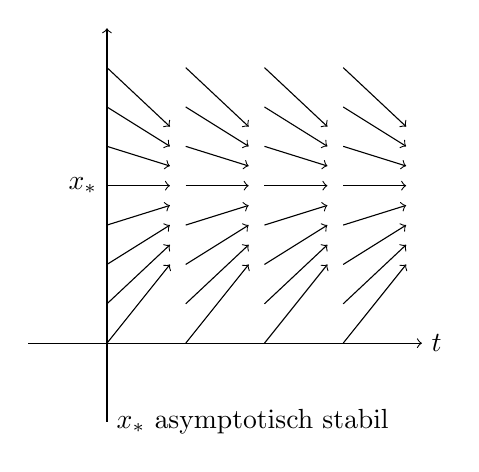
\begin{tikzpicture}
		\draw[->] (0,-1) node[right]{$x_*$ asymptotisch stabil} -- (0,4) ;
		\draw[->] (-1,0) -- (4,0) node[right]{$t$};
		\foreach \i in {0,...,3}
		{
			\foreach \j in {0,...,7}
			{
				\draw[->] (\i,\j / 2) -- (\i + 0.8,\j / 4 + 1) ;
			}
		}
		\draw (0,2) node[left]{$x_*$};
		\end{tikzpicture}
		%
		\hspace{0.1\textwidth}%
		%
		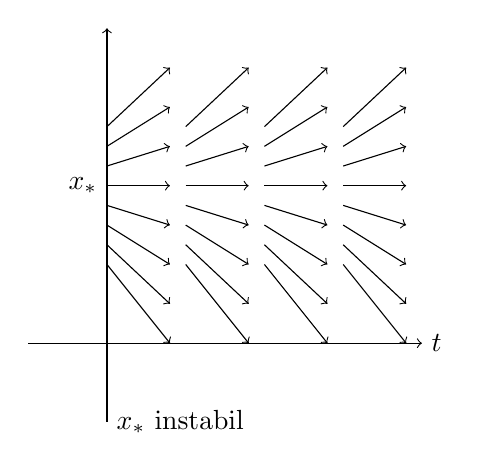
\begin{tikzpicture}
		\draw[->] (0,-1) node[right]{$x_*$ instabil} -- (0,4) ;
		\draw[->] (-1,0) -- (4,0) node[right]{$t$};
		\foreach \i in {0,...,3}
		{
			\foreach \j in {0,...,7}
			{
				\draw[->] (\i,\j / 4 + 1) -- (\i + 0.8,\j / 2) ;
			}
		}
		\draw (0,2) node[left]{$x_*$};
		\end{tikzpicture}
	\end{center}
	Man erkennt an den Bildern, dass die asymptotische Stabilität von $x_*$ mit der Ableitung von $f$ in (der Nähe von) $x_*$ zusammenhängt. 
\end{bsp}


\begin{satz}[{{\cite[3.30]{deuflhard_bornemann:2008}}}]
	Sei $x_* \in \Omega_0$ Fixpunkt von $x' = f(x)$, und $f$ sei stetig differenzierbar. Falls
	\begin{equation*}
	\nu(Df(x_*)) < 0
	\end{equation*}
	so ist $x_*$ asymptotisch stabiler Fixpunkt
\end{satz}

\textbf{Erinnerung:} $\nu$ ist die Spektralabzisse, der größte Realteil aller Eigenwerte.

\textbf{Zwischenfazit:} Um die asymptotische Stabilität von Fixpunkten zu untersuchen, reicht es, sich die Linearisierung um $ x_* $ anzuschauen!

Wir betrachten jetzt zusätzlich die um $ x_* $ linearisierte Differentialgleichung
\begin{equation}\label{Gleichung:Linearisierte-Differentialgleichung}
(x-x_*)' = x' = Df(x_*)(x-x_*).
\end{equation}

\begin{idea}
	Wenn $Df(x_*)$ das Stabilitätsverhalten von $x_*$ qualitativ richtig beschreibt, dann enthält die \emph{lineare} Gleichung~\eqref{Gleichung:Linearisierte-Differentialgleichung}
	vielleicht schon alle \enquote{schwierigen} (im Sinne der Stabilität) Aspekte von $ x'=f(x)$ in der Nähe von $ x_* $?
\end{idea}

Betrachte ein beliebiges Einschrittverfahren. Sei
\begin{itemize}
	\item $\Psi^\tau$ diskreter Fluss für das Ausgangsproblem
	\item $\Psi_*^\tau$ diskreter Fluss für das linearisierte Problem $x'=Df(x_*)(x-x_*)$.
\end{itemize}

\begin{definition}
	Ein Einschrittverfahren heißt \begriff{invariant gegen Linearisierung} um einen Fixpunkt $x_*$, wenn
	\begin{enumerate}
		\item $\Psi^\tau x_*=x_*\ \forall\tau>0$ ($\tau$ zulässig)
		$\qquad \rightarrow$ der Fixpunkt der Differentialgleichung ist auch
		Fixpunkt des numerischen Verfahrens für die nichtlineare Gleichung.
		
		\item $\Psi_*^\tau x = x_* + R(\tau Df(x_*))(x-x_*)$ mit einer rationalen Funktion $R$, die nur vom Verfahren abhängt; d.h. für das linearisierte Problem degeneriert das Verfahren zu einer rationalen Approximation der Exponentialfunktion.
		
		\item $D_x\Psi^\tau x\vert_{x=x_*}=\Psi^\tau_*$ für alle zulässigen $\tau$ $\qquad \rightarrow$ $\Psi^\tau_*$ ist Linearisierung von $\Psi^\tau$.
	\end{enumerate}
\end{definition}

Zum Beispiel sind alle expliziten RK-Verfahren in diesem Sinne invariant. Solch ein Verfahren heißt $A$-stabil, falls $R$ $A$-stabil ist.

Invariante Verfahren retten den Zusammenhang zwischen der asymptotischen Stabilität eines Fixpunkts $x_*$ und der Linearisierung dort ins Diskrete:

\begin{satz}[{{\cite[6.23]{deuflhard_bornemann:2008}}}]
	Sei $\Psi^\tau$, $\Psi^\tau_*$ ein gegen Linearisierung invariantes Einschrittverfahren. Sei $\tau_c\geq 0$ die maximale Schrittweite, so dass $\Psi^\tau_*$ die asymptotische Stabilität erbt. Dann ist $x_*$ asymptotisch stabiler Fixpunkt der Rekursion
	\begin{equation*}
		x_{n+1} = \Psi^\tau x_n\qquad n=0,1,2,\hdots
	\end{equation*}
	für alle $\tau<\tau_c$.
\end{satz}

\begin{bsp}
	Skalare Differentialgleichung $x' = \lambda(1-x^2) \qquad (\lambda > 0)$
	\begin{itemize}
		\item Fixpunkte: $ x_s = 1$ (asymptotisch stabil) und $x_u = -1$ instabil	
		\item Linearisierte Gleichung in $x_s$:
		\begin{equation*}
			x' = f'(x_s)(x-x_s) = -2\lambda x_s(x-x_s) = -2\lambda(x-1)
		\end{equation*}
		\item Explizites Euler-Verfahren dafür stabil, wenn $\tau< 1/\lambda$
		\item Es folgt: $x_s$ ist auch asymptotisch stabiler Fixpunkt des expliziten Euler-Verfahrens für die nichtlineare Gleichung
		\begin{equation*}
			x_{n+1} = x_n + \tau f(x_n) = x_n + \tau\lambda(1-x_n^2).
		\end{equation*}
		Aber wie gesagt nur falls $\tau< 1/\lambda$.
	\end{itemize}
	Und nicht vergessen: $x_s$ ist nur dann Attraktor, wenn man nah genug dran startet. Für dieses Beispiel heißt das:
	\begin{itemize}
		\item Kontinuierlich: $x_0>-1$
		\item Euler: $x_0\in[0, \frac{5}{4}]$.
	\end{itemize}
\end{bsp}

\subsection{Linear-implizite Runge--Kutta-Verfahren}

\begin{idea}
	Behandle nur den linearen Teil von $f$ implizit.
\end{idea}

Für festes $\bar{x} \in \Omega_0$ schreibe die Differentialgleichung als
\begin{equation*}
	x'(t) = Jx(t) + (f(x(t)) - Jx(t)) \qquad J=Df(\bar{x})\in\R^{d\times d}
\end{equation*}
Hier ist $\bar{x}$ beliebig; in der Praxis linearisiert man um den Zustand
zum vorigen Zeitschritt.

Wende das implizite Euler-Verfahren auf den ersten Term an, und das explizite Euler-Verfahren auf den Rest.
\begin{equation*}
\Psi^\tau x = \xi + \tau(f(x)-Jx),\qquad \xi = x+\tau J\xi
\end{equation*}
Das ist das linear-implizite oder \begriff{semi-implizite Euler-Verfahren}.
Wir haben nur ein \textit{lineares} Gleichungssystem pro Schritt, aber sind trotzdem $A$-stabil.

Betrachten wir nun allgemein \begriff{linear-implizite Runge-Kutta-Verfahren}
\begin{equation*}
\Psi^\tau x = x + \tau \sum_{j=1}^s b_j k_j
\end{equation*}
\begin{equation*}
k_i = J\Big(x+\tau\sum_{j=1}^i \beta_{ij} k_j\Big)
+ \bigg[ f\Big(x+\tau\sum_{j=1}^{i-1} \alpha_{ij} k_j\Big)
- J\Big(x+\tau\sum_{j=1}^{i-1} \alpha_{ij} k_j\Big)\bigg]
\end{equation*}
für $i=1,\dots,s$.

\begin{hinw}
	Der obere Summationsindex des impliziten Teils ist $i$, nicht $s$.
\end{hinw}

Dadurch kann der Phasenfluss durch wiederholtes Lösen \textit{linearer} Gleichungssysteme berechnet werden.
\begin{enumerate}
	\item $J = Df(x)$
	\item $\displaystyle (I-\tau\beta_{ii}J)k_i = \tau\sum_{j=1}^{i-1}(\beta_{ij}-\alpha_{ij})Jk_j + f\Big(x + \tau\sum_{j=1}^{i-1} \alpha_{ij} k_j\Big)$ für $i=1,\dots,s$
	\item $\displaystyle \Psi^\tau x = x + \tau\sum_{j=1}^{s} b_j k_j$
\end{enumerate}
Solche Verfahren heißen \begriff{lineare-implizite RK-Verfahren} oder \begriff{Rosenbrock-Verfahren}.


Koeffizienten: $A=(\alpha_{ij})\in\R^{s\times s},\ B=(\beta_{ij})\in\R^{s\times s},\  b=(b_1\hdots,b_s)$

Wählt man die $\beta_{ii}$ alle gleich, so haben die $s$ Gleichungssysteme in (2) alle die gleiche Matrix und es reicht eine LR-Zerlegung, um alle $s$ Gleichungssysteme zu lösen.

Die Frage, ob sich die linearen Gleichungssysteme tatsächlich immer lösen lassen, ist einfacher als für den allgemeinen impliziten Fall:
\begin{lemma}
	Sei $\beta \geq 0$ und $J\in\R^{d\times d}$. Die Matrix $I-\tau\beta J$ ist für alle $0\leq \tau\leq \tau_*$ invertierbar. Dabei hängt $\tau_*$ von der Spektralabzisse $\nu(J)$ ab:
	\begin{equation*}
	\tau_* = \infty\text{ für } \nu(J)\leq 0, \qquad \tau_* =  \frac{1}{\beta\nu(J)} \text{ für }	\nu(J) > 0.
	\end{equation*}
\end{lemma}
\begin{proof}
	Zu zeigen: Unter den gegebenen Voraussetzungen hat $I-\tau\beta J$ nicht den Eigenwert $0$. Nach Satz~\eqref{thm:spektrale_aequivarianz} über rationale Funktionen ist aber
	\begin{equation*}
	\sigma(I-\tau\beta J) = 1-\tau\beta\sigma(J).
	\end{equation*}
	Deshalb zu zeigen: $J$ hat keinen Eigenwert $\lambda$ mit $1-\tau\beta\lambda = 0$.\\
	\begin{enumerate}[label=Fall \arabic*:, leftmargin=*]
		\item $\nu(J) \leq 0$, d.h. insbesondere $\Re(\lambda)\leq 0$:
		\begin{equation*}
		\Re(1-\tau\beta\lambda) = 1-\tau\beta \Re(\lambda) \geq 1 \quad  \Rightarrow \quad 1-\tau\beta\lambda \neq 0
		\end{equation*}
		\item $0<\Re(\lambda)\leq \nu(J)$:
		\begin{equation*}
		\Re(1-\tau\beta\lambda) = 1 - \tau \beta \Re(\lambda) \geq 1 - \tau\beta\nu(J)
		\end{equation*}
		Also $>0$ wenn $\tau < \frac{1}{\beta\nu(J)}$
	\end{enumerate}
\end{proof}

Der Satz sagt also: Die steifen Anteile der Differentialgleichung (d.h. die nichtpositiven Eigenwert von $J$) beeinflussen nicht die Lösbarkeit des Gleichungssystems.

Für autonome \textit{lineare} Probleme ist das Verfahren offensichtlich äquivalent zum impliziten Runge-Kutta-Verfahren $(b, (\beta_{ij}))$.  Es hat also die selbe Stabilitätsfunktion.

Die Konstruktion der Bedingungsgleichungen funktioniert ähnlich wie bei expliziten RK-Verfahren.
